\documentclass{beamer}
\usepackage[utf8]{inputenc}
\usepackage{graphicx, epsfig}
\usepackage{amsmath,mathrsfs,amsfonts,amssymb}
%\usepackage{subfig}
\usepackage{floatflt}
\usepackage{epic,ecltree}
\usepackage{mathtext}
\usepackage{fancybox}
\usepackage{fancyhdr}
\usepackage{multirow}
\usepackage{enumerate}
\usepackage{epstopdf}
\usepackage{multicol}
\usepackage{algorithm}
\usepackage[noend]{algorithmic}
\usepackage{tikz}
\usepackage{blindtext}
\usetheme{default}%{Singapore}%{Warsaw}%{Warsaw}%{Darmstadt}
\usecolortheme{default}
\setbeamerfont{title}{size=\Huge}
\setbeamertemplate{footline}[page number]{}


\makeatletter
\newcommand\HUGE{\@setfontsize\Huge{35}{40}}
\makeatother    

\setbeamerfont{title}{size=\HUGE}
\beamertemplatenavigationsymbolsempty

% latin bold lower
\newcommand{\ba}{\mathbf{a}} 
\newcommand{\bc}{\mathbf{c}} 
\newcommand{\be}{\mathbf{e}} 
\newcommand{\bh}{\mathbf{h}} 
\newcommand{\bp}{\mathbf{p}} 
\newcommand{\bt}{\mathbf{t}} 
\newcommand{\bs}{\mathbf{s}} 
\newcommand{\bu}{\mathbf{u}} 
\newcommand{\bv}{\mathbf{v}} 
\newcommand{\bw}{\mathbf{w}} 
\newcommand{\bx}{\mathbf{x}} 
\newcommand{\by}{\mathbf{y}} 
\newcommand{\bz}{\mathbf{z}} 

% latin bold upper
\newcommand{\bA}{\mathbf{A}} 
\newcommand{\bB}{\mathbf{B}} 
\newcommand{\bC}{\mathbf{C}} 
\newcommand{\bI}{\mathbf{I}} 
\newcommand{\bL}{\mathbf{L}} 
\newcommand{\bM}{\mathbf{M}} 
\newcommand{\bQ}{\mathbf{Q}} 
\newcommand{\bT}{\mathbf{T}} 
\newcommand{\bU}{\mathbf{U}} 
\newcommand{\bV}{\mathbf{V}} 
\newcommand{\bW}{\mathbf{W}} 
\newcommand{\bX}{\mathbf{X}} 
\newcommand{\bY}{\mathbf{Y}} 
\newcommand{\bZ}{\mathbf{Z}} 

% latin cal upper
\newcommand{\cG}{\mathcal{G}} 
\newcommand{\cL}{\mathcal{L}} 
\newcommand{\cN}{\mathcal{N}} 
\newcommand{\cS}{\mathcal{S}} 
\newcommand{\cT}{\mathcal{T}} 
\newcommand{\cW}{\mathcal{W}} 
\newcommand{\cX}{\mathcal{X}} 
\newcommand{\cZ}{\mathcal{Z}} 

% latin bb upper
\newcommand{\bbE}{\mathbb{E}} 
\newcommand{\bbI}{\mathbb{I}} 
\newcommand{\bbP}{\mathbb{P}} 
\newcommand{\bbR}{\mathbb{R}} 

% greek bold lower
\newcommand{\bepsilon}{\boldsymbol{\epsilon}} 
\newcommand{\btheta}{\boldsymbol{\theta}} 
\newcommand{\blambda}{\boldsymbol{\lambda}} 
\newcommand{\bpi}{\boldsymbol{\pi}} 
\newcommand{\bmu}{\boldsymbol{\mu}} 
\newcommand{\bsigma}{\boldsymbol{\sigma}} 
\newcommand{\bphi}{\boldsymbol{\phi}} 

% greek bold upper
\newcommand{\bSigma}{\boldsymbol{\Sigma}} 

\DeclareMathOperator*{\argmin}{arg\,min}
\DeclareMathOperator*{\argmax}{arg\,max}

\newcommand{\createdgmtitle}[1]{\title[\hbox to 56mm{Deep Generative Models  \hfill\insertframenumber\,/\,\inserttotalframenumber}]
	{\vspace{1.5cm} \\ Deep Generative Models \\ {\Huge Lecture #1}}
	\author{Roman Isachenko}
	\institute{
	Moscow Institute of Physics and Technology
	} 
	\date{Autumn, 2021}
}

\newcommand\myfootnote[1]{%
  \tikz[remember picture,overlay]
  \draw (current page.south west) +(1in + \oddsidemargin,0.5em)
  node[anchor=south west,inner sep=0pt]{\parbox{\textwidth}{%
      \rlap{\rule{10em}{0.4pt}}\raggedright\scriptsize \textit{#1}}};}

\newcommand\myfootnotewithlink[2]{%
  \tikz[remember picture,overlay]
  \draw (current page.south west) +(1in + \oddsidemargin,0.5em)
  node[anchor=south west,inner sep=0pt]{\parbox{\textwidth}{%
      \rlap{\rule{10em}{0.4pt}}\raggedright\scriptsize\href{#1}{\textit{#2}}}};}
\createdgmtitle{2}

\usepackage{tikz}

\usetikzlibrary{arrows,shapes,positioning,shadows,trees}
%--------------------------------------------------------------------------------
\begin{document}
%--------------------------------------------------------------------------------
\begin{frame}[noframenumbering,plain]
	%\thispagestyle{empty}
	\titlepage
\end{frame}
%=======
\begin{frame}{Recap of previous lecture}
	We are given i.i.d. samples $\{\bx_i\}_{i=1}^n \in X$ (e.g. $X = \bbR^m$) from unknown distribution $\pi(\bx)$.

	\begin{block}{Goal}
		We would like to learn a distribution $\pi(\bx)$ for 
		\begin{itemize}
		    \item evaluating $\pi(\bx)$ for new samples (how likely to get object $\bx$?);
		    \item sampling from $\pi(\bx)$ (to get new objects $\bx \sim \pi(\bx)$).
		\end{itemize}
	\end{block}
	Instead of searching true $\pi(\bx)$ over all probability distributions, learn function approximation $p(\bx | \btheta) \approx \pi(\bx)$.
	\begin{block}{Divergence}
		\begin{itemize}
			\item $D(\pi || p) \geq 0$ for all $\pi, p \in \cS$;
			\item $D(\pi || p) = 0$ if and only if $\pi \equiv p$.
		\end{itemize}
	\end{block}
	\begin{block}{General divergence minimization task}
		\vspace{-0.3cm}
		\[
		\min_{\btheta} D(\pi || p).
		\]
	\end{block}
\end{frame}
%=======
\begin{frame}{Recap of previous lecture}
	\begin{block}{Forward KL}
		\vspace{-0.2cm}
		\[
		KL(\pi || p) = \int \pi (\bx) \log \frac{\pi(\bx)}{p(\bx | \btheta)} d \bx \rightarrow \min_{\btheta}
		\]
	\end{block}
	\begin{block}{Reverse KL}
		\vspace{-0.2cm}
		\[
		KL(p || \pi) = \int p (\bx| \btheta) \log \frac{p(\bx| \btheta)}{\pi(\bx)} d \bx \rightarrow \min_{\btheta}
		\]
	\end{block}
	
	\begin{block}{Maximum likelihood estimation (MLE)}
		\vspace{-0.5cm}
		\[
		\btheta^* = \argmax_{\btheta} p(\bX | \btheta) = \argmax_{\btheta} \prod_{i=1}^n p(\bx_i | \btheta) = \argmax_{\btheta} \sum_{i=1}^n \log p(\bx_i | \btheta).
		\]
		\vspace{-0.1cm}
	\end{block}
	Maximum likelihood estimation is equivalent to minimization of the Monte-Carlo estimate of forward KL.
\end{frame}
%=======
\begin{frame}{Recap of previous lecture}
	\begin{block}{Likelihood as product of conditionals}
		Let $\bx = (x_1, \dots, x_m)$, $\bx_{1:j} = (x_1, \dots, x_j)$. Then 
		\[
		p(\bx | \btheta) = \prod_{j=1}^m p(x_j | \bx_{1:j - 1}, \btheta); \quad 
		\log p(\bx | \btheta) = \sum_{j=1}^m \log p(x_j | \bx_{1:j - 1}, \btheta).
		\]
	\end{block}
	\vspace{-0.3cm}
	\begin{block}{MLE problem for autoregressive model}
		\vspace{-0.5cm}
		\[
		\btheta^* = \argmax_{\btheta} p(\bX | \btheta) = \argmax_{\btheta} \sum_{i=1}^n \sum_{j=1}^m \log p(x_{ij} | \bx_{i, 1:j - 1}\btheta).
		\]
		\vspace{-0.5cm}
	\end{block}
	\begin{block}{Sampling}
		\vspace{-0.5cm}
		\[
			\hat{x}_1 \sim p(x_1 | \btheta), \quad \hat{x}_2 \sim p(x_2 | \hat{x}_1, \btheta), \dots, \quad \hat{x}_m \sim p(x_m | \hat{\bx}_{1:m-1}, \btheta)
		\]
		New generated object is $\hat{\bx} = (\hat{x}_1, \hat{x}_2, \dots, \hat{x}_m)$.
	\end{block}
\end{frame}
%=======
\begin{frame}{Recap of previous lecture}
	\begin{block}{Autoregressive MLP}
		\vspace{-0.3cm}
 		\begin{figure}
		     \centering
		     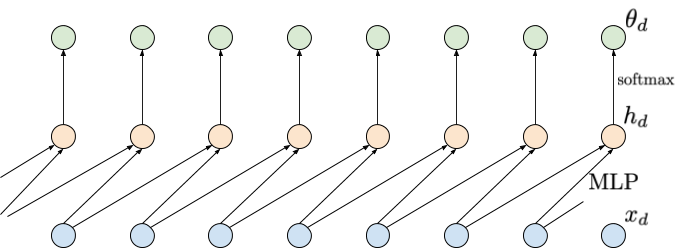
\includegraphics[width=0.75\linewidth]{figs/sequential_MLP}
		 \end{figure}
	\end{block}
	\begin{block}{Autoregressive RNN}
	   	\vspace{-0.3cm}
		\begin{figure}
		   \centering
		   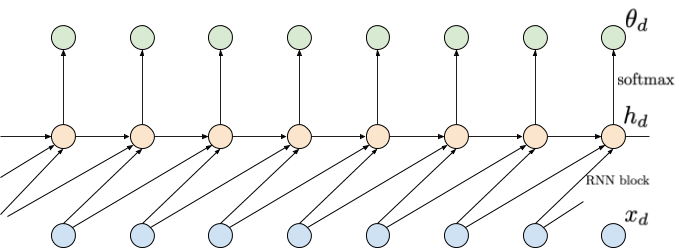
\includegraphics[width=0.75\linewidth]{figs/sequential_RNN}
		\end{figure}
	\end{block}
	 \myfootnotewithlink{https://jmtomczak.github.io/blog/2/2\_ARM.html}{image credit: https://jmtomczak.github.io/blog/2/2\_ARM.html}
\end{frame}
%=======
\begin{frame}{Char RNN}
	Model tries to predict the next token (single letter) from previous context.
	\begin{minipage}[t]{0.55\columnwidth}
		\begin{figure}
			\centering
			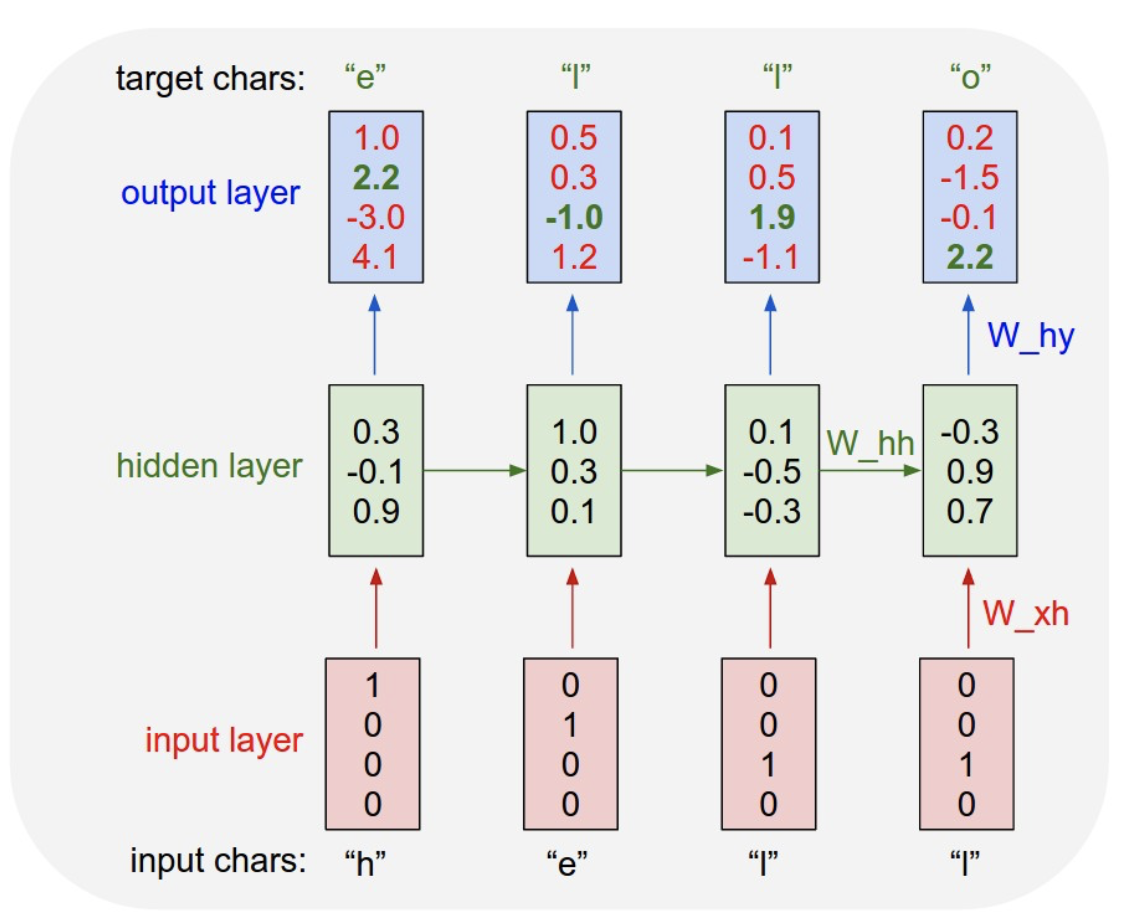
\includegraphics[width=1.0\linewidth]{figs/char_rnn.png}
		\end{figure}
	\end{minipage}%
	\begin{minipage}[t]{0.44\columnwidth}
		\begin{figure}
			\centering
			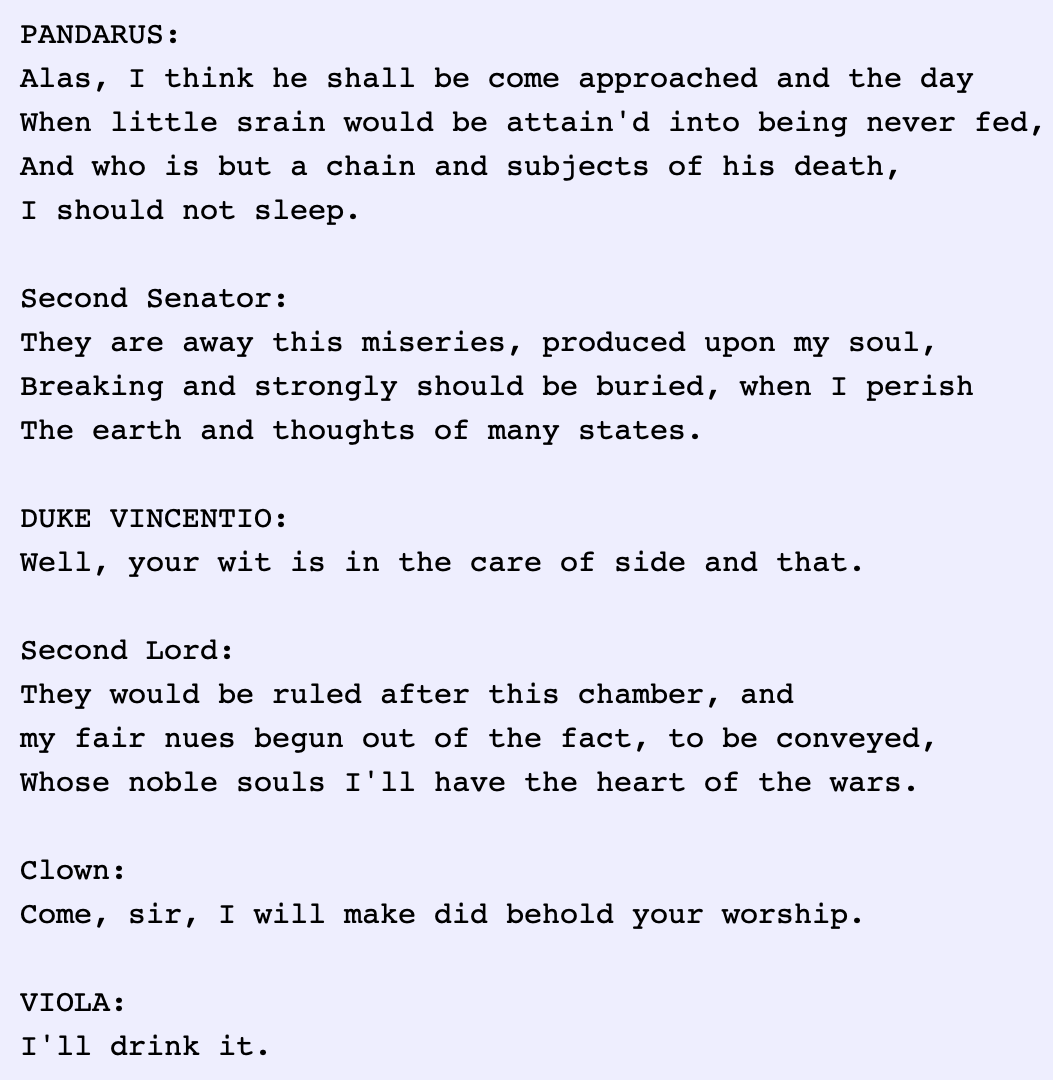
\includegraphics[width=1.0\linewidth]{figs/char_rnn_output.png}
		\end{figure}
	\end{minipage}
\myfootnotewithlink{http://karpathy.github.io/2015/05/21/rnn-effectiveness/}{image credit: http://karpathy.github.io/2015/05/21/rnn-effectiveness}
\end{frame}
%=======
\begin{frame}{Autoregressive models}
		\begin{itemize}
			\item Convolutions could be used for autoregressive models, but they have to be \textbf{causal}. \\
			\item Try to find and understand the difference between Conv A/B.
		    \begin{figure}
		        \centering
		        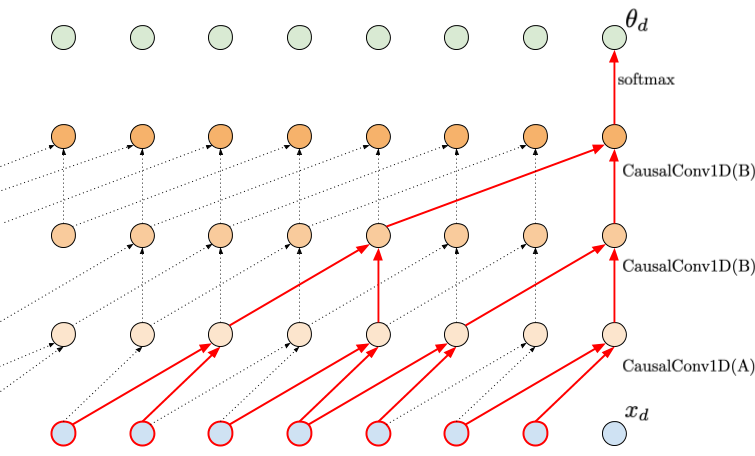
\includegraphics[width=0.7\linewidth]{figs/sequential_CNN}
		    \end{figure}
		    \item Could learn long-range dependecies.
		    \item Do not suffer from gradient issues.
		    \item Easy to estimate probability for given input, but hard generation of new samples (the sequential process).
	   	\end{itemize}
	    \myfootnotewithlink{https://jmtomczak.github.io/blog/2/2\_ARM.html}{image credit: https://jmtomczak.github.io/blog/2/2\_ARM.html}
\end{frame}
%=======
\begin{frame}{MADE}
	\begin{itemize}
		\item Vanila autoencoder is not a generative model.
		\item Let mask the weight matrices to make the model generative: $\bW_M = \bW \cdot \bM$.
		\begin{figure}
		    \centering
		    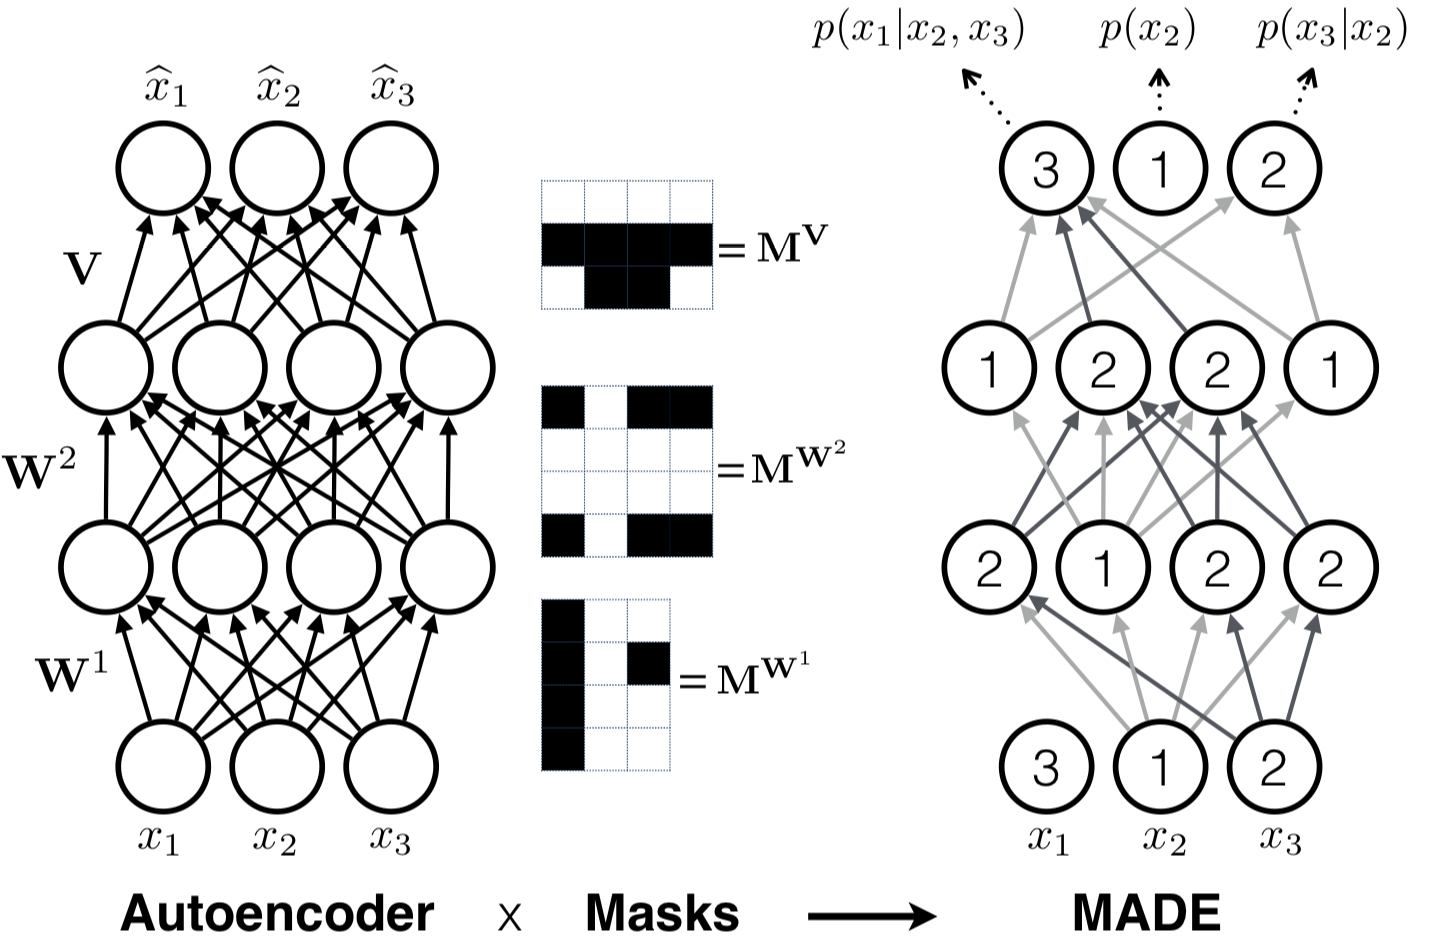
\includegraphics[width=0.7\linewidth]{figs/made}
		\end{figure}
		\item The question is how to create matrices $\bM$ which produce the autoregressive property?
	\end{itemize}
	\myfootnotewithlink{https://arxiv.org/abs/1502.03509}{Germain M. et al. Made: Masked autoencoder for distribution estimation, 2015}
\end{frame}
%=======
\begin{frame}{MADE}
		\begin{minipage}[t]{0.65\columnwidth}
		    \vspace{-0.5cm}
			\begin{block}{Masks generation}
				\begin{itemize}
					\item Define the ordering of input elements from 1 to $m$.
					\item Assign the random number $k$ from 1 to $m - 1$ to each hidden unit. The number gives the
					maximum value of input units to which the unit can be connected.
					\item Connect each hidden unit with number $k$ with the previous layer units which has the number is \textbf{less or equal} than~$k$.
					\item Connect each output unit with number $k$ with the previous layer units which has the number is \textbf{less} than $k$.
				\end{itemize}
			\end{block}
		\end{minipage}%
		\begin{minipage}[t]{0.33\columnwidth}
			\vspace{2cm}
			\begin{figure}
				\centering
				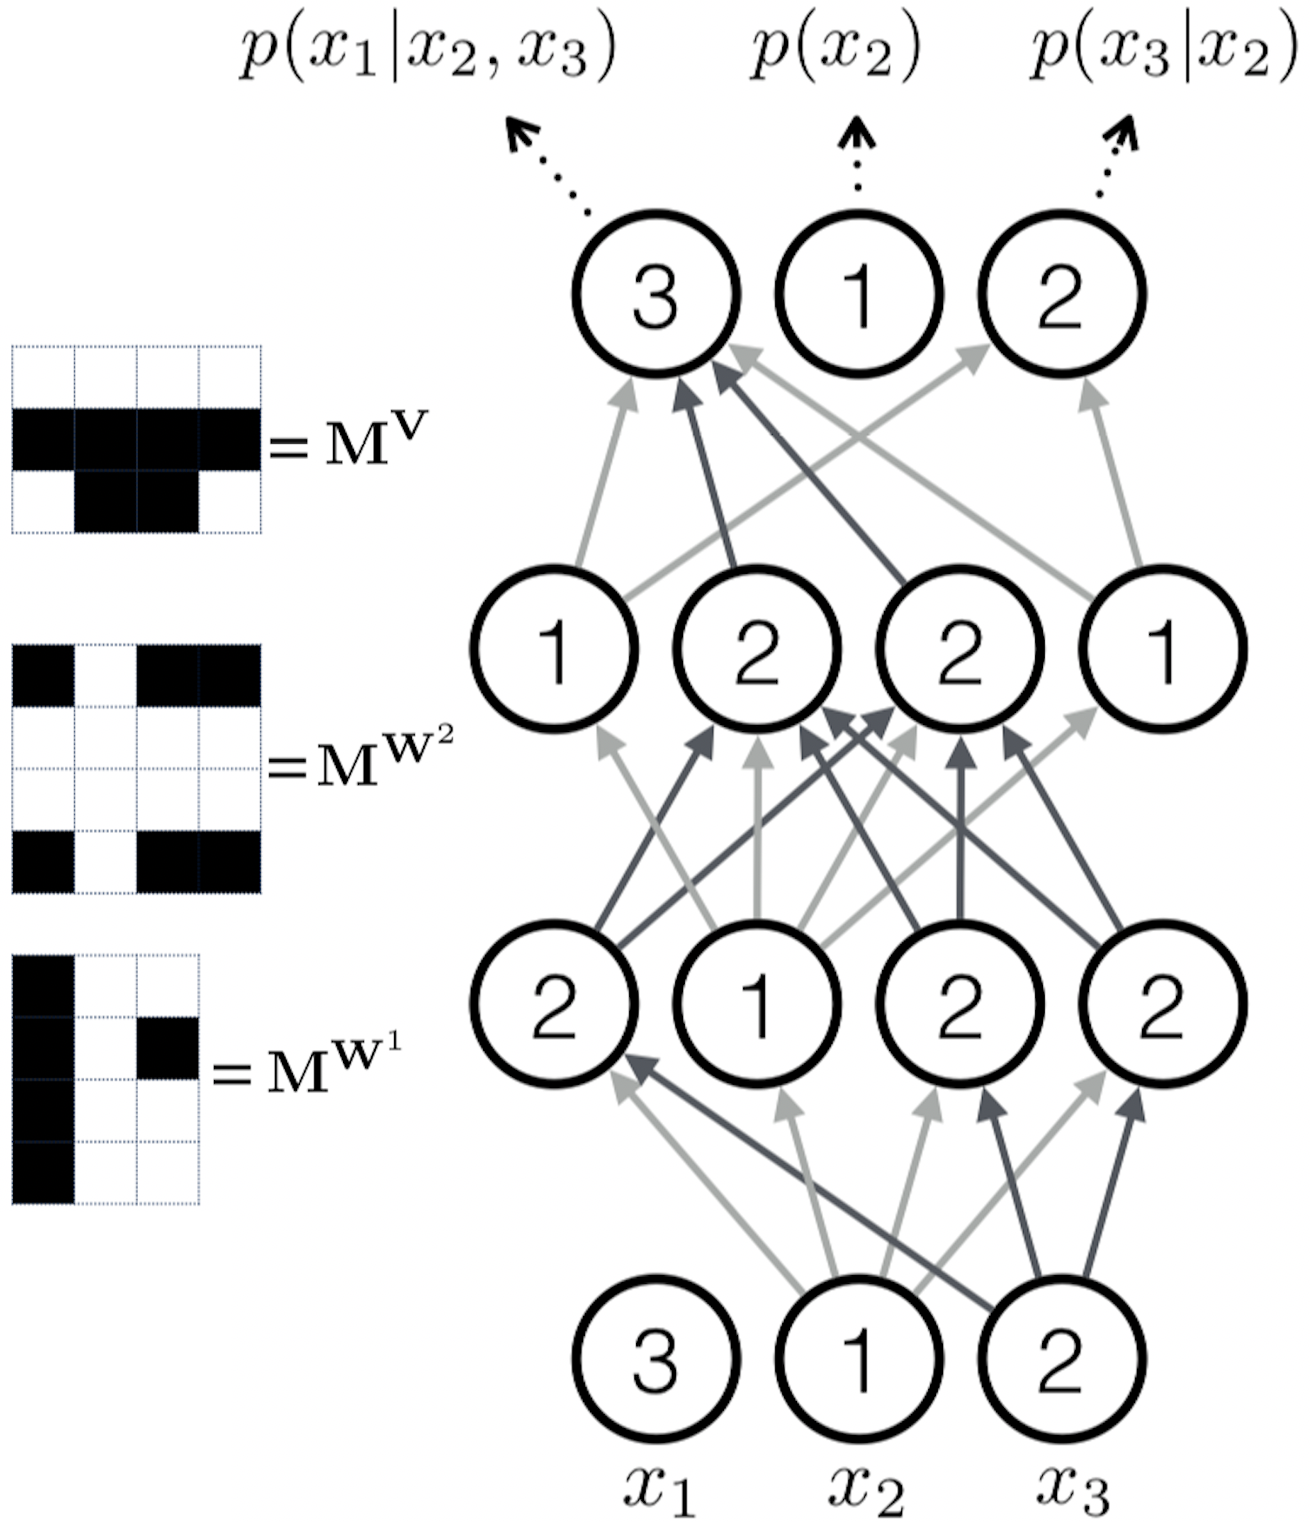
\includegraphics[width=1.0\linewidth]{figs/made2}
			\end{figure}
		\end{minipage}
	\myfootnotewithlink{https://arxiv.org/abs/1502.03509}{Germain M. et al. Made: Masked autoencoder for distribution estimation, 2015}
\end{frame}
%=======
\begin{frame}{MADE}
	\begin{block}{Possible variations}
		\begin{itemize}
			\item Order agnostic training (missing values in partially observed input vectors can be imputed efficiently);
			\item Connectivity-agnostic training (cheap ensembling).
		\end{itemize}
	\end{block}
	\vspace{-0.3cm}
	\begin{minipage}[t]{0.59\columnwidth}
		\begin{figure}
			  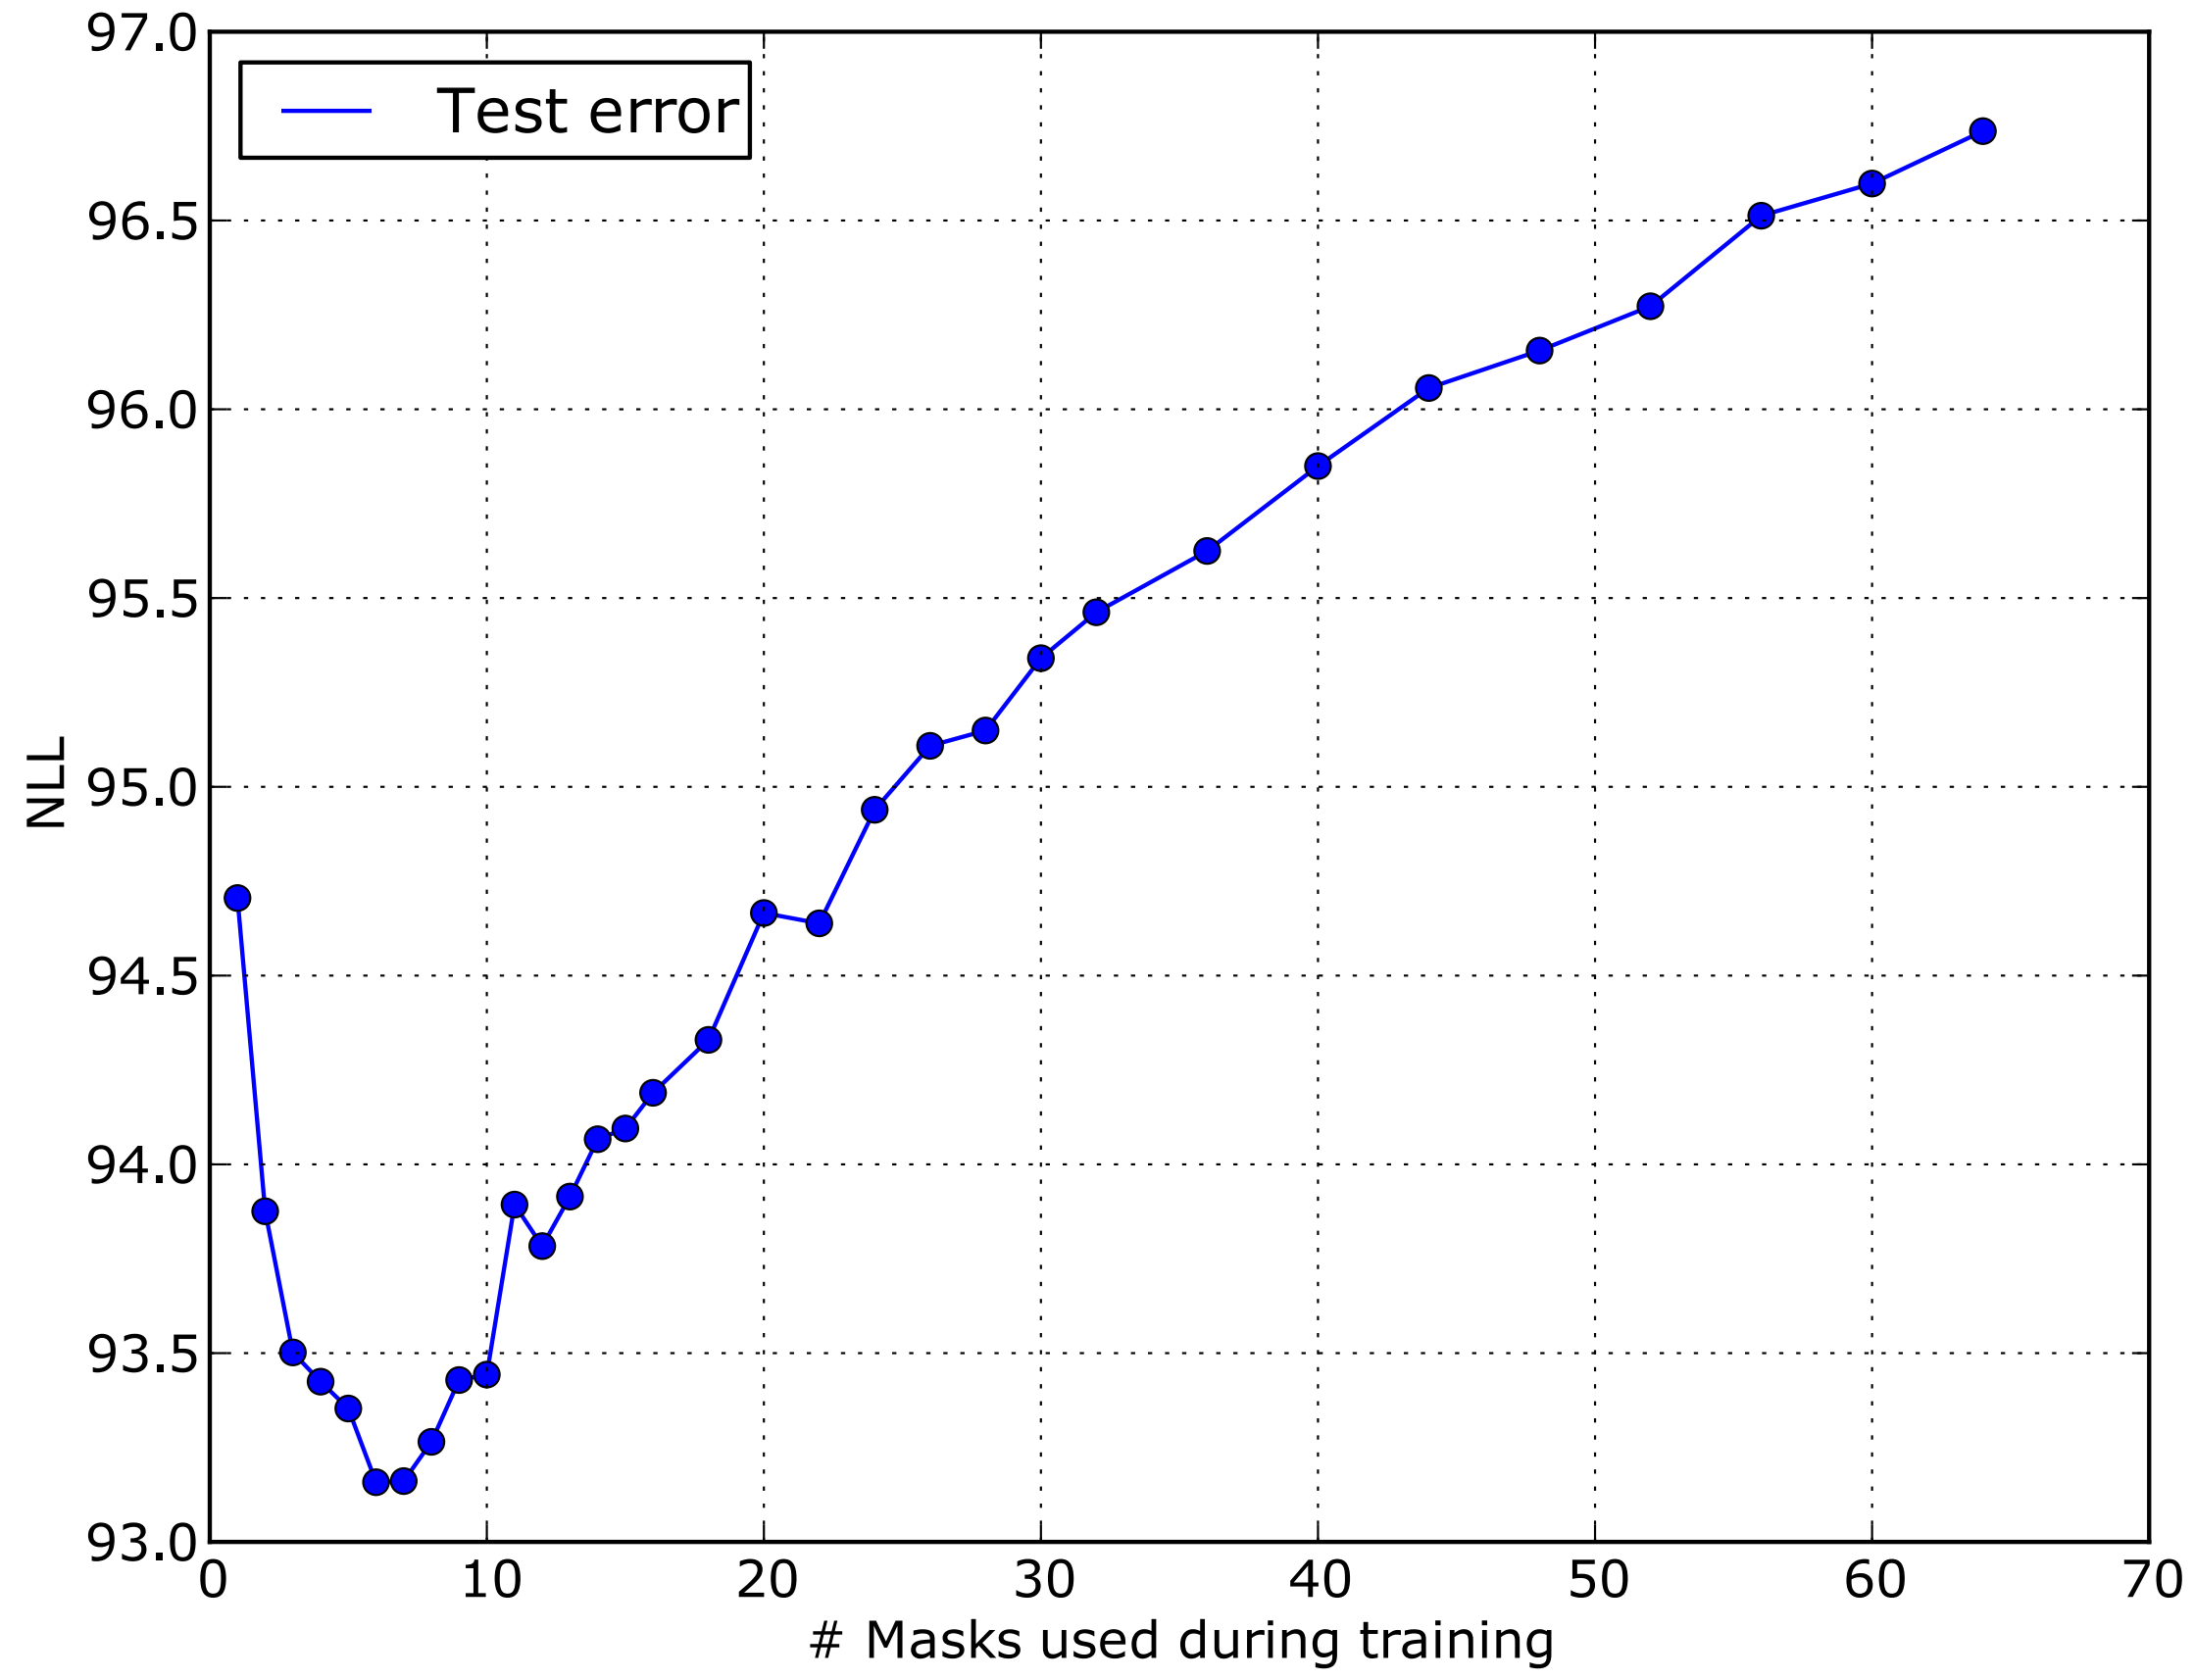
\includegraphics[width=\linewidth]{figs/made_nmasks}
		\end{figure}
	\end{minipage}%
	\begin{minipage}[t]{0.41\columnwidth}
		\begin{figure}
	  		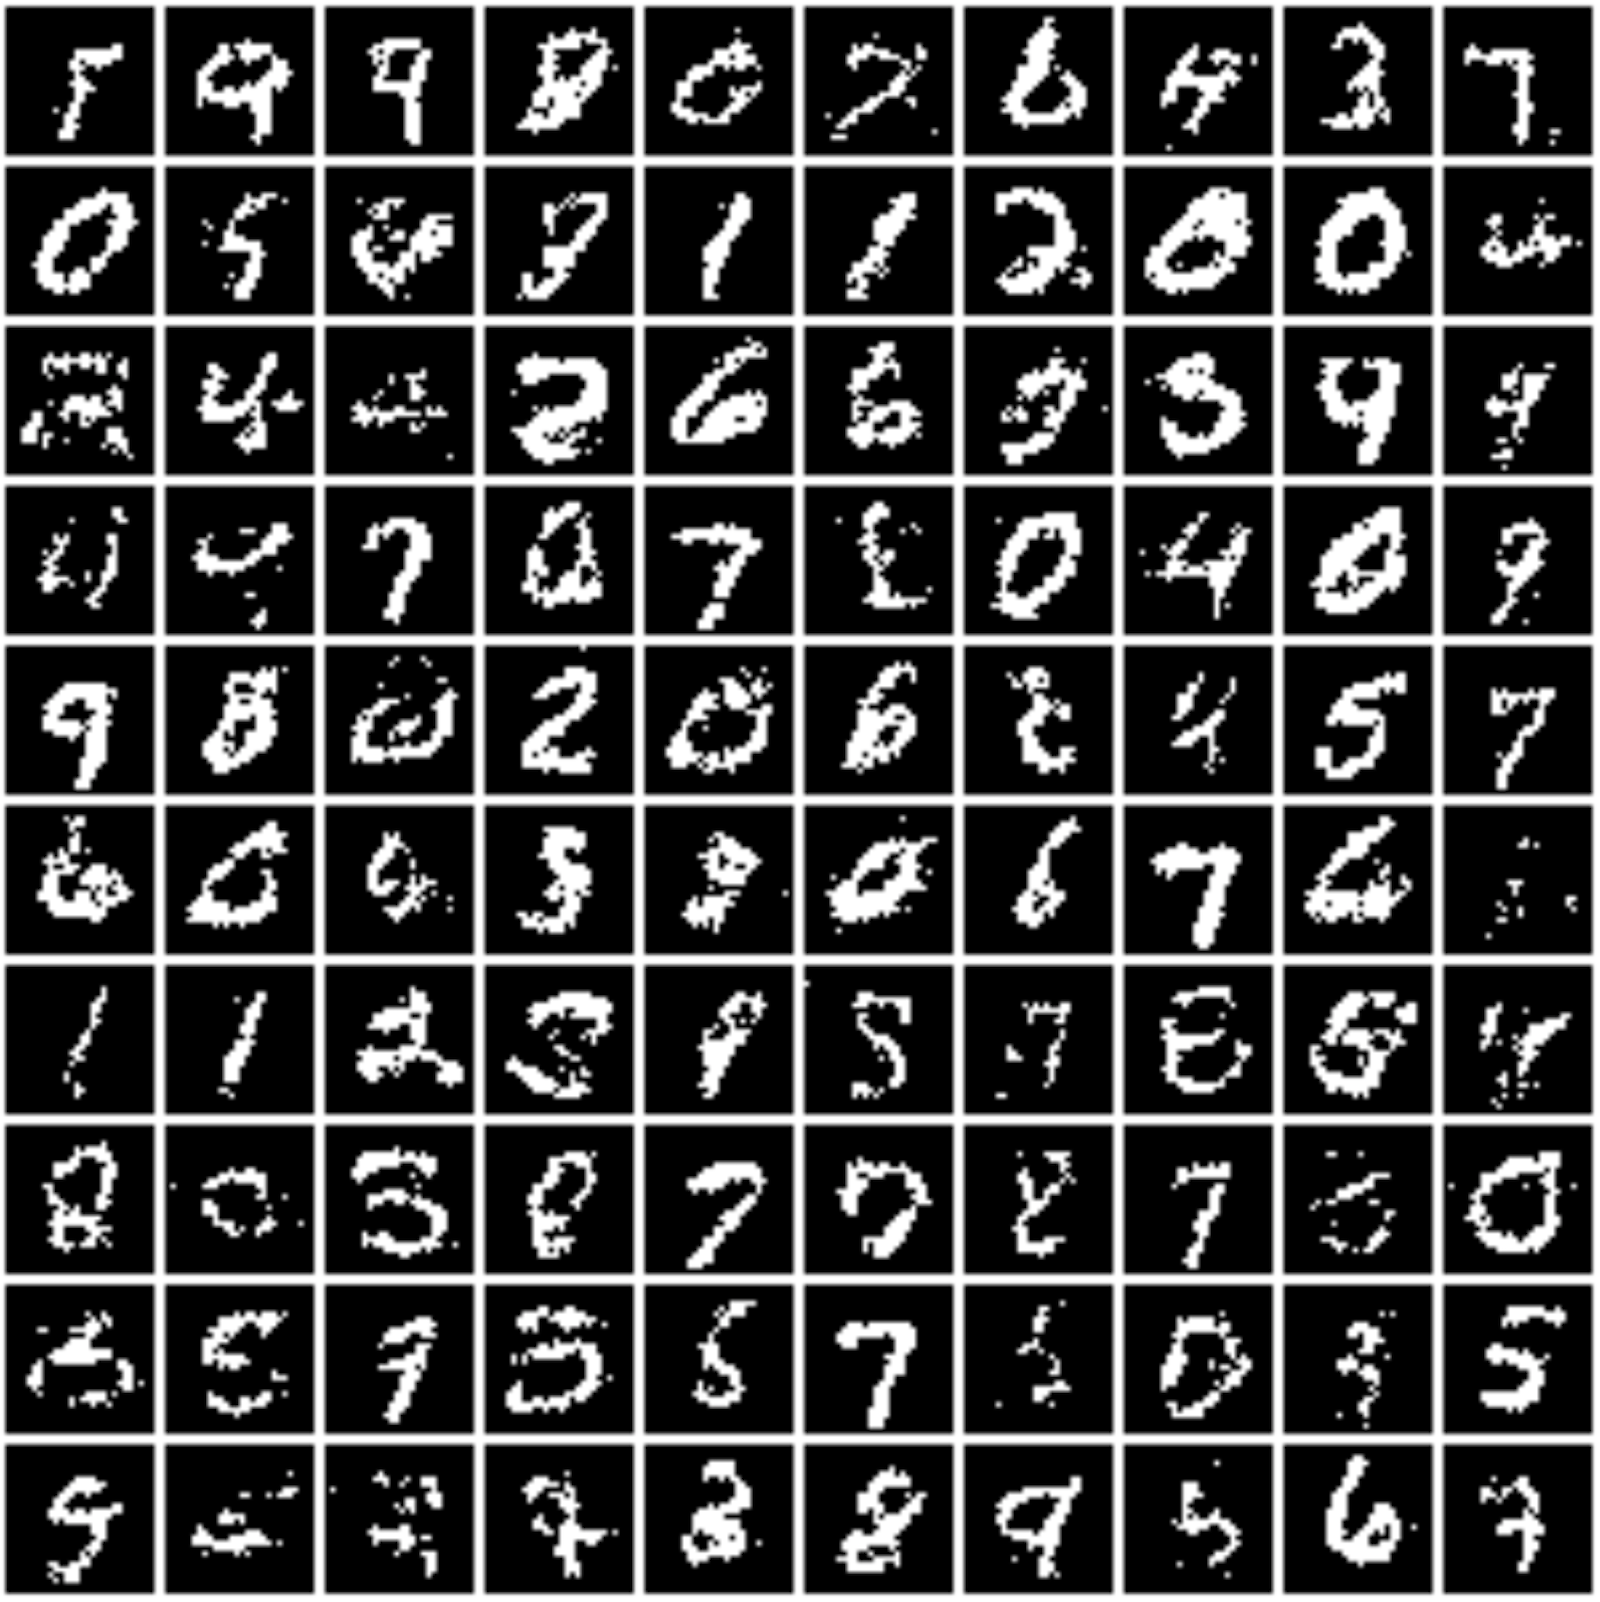
\includegraphics[width=\linewidth]{figs/made_results}
		\end{figure}
	\end{minipage}
	\myfootnotewithlink{https://arxiv.org/abs/1502.03509}{Germain M. et al. Made: Masked autoencoder for distribution estimation, 2015}
\end{frame}
%=======%=======
\begin{frame}{WaveNet}
	\begin{block}{Goal}
		Efficient generation of raw audio waveforms with natural sounds.
	\end{block}
	\begin{figure}
	  \centering
	  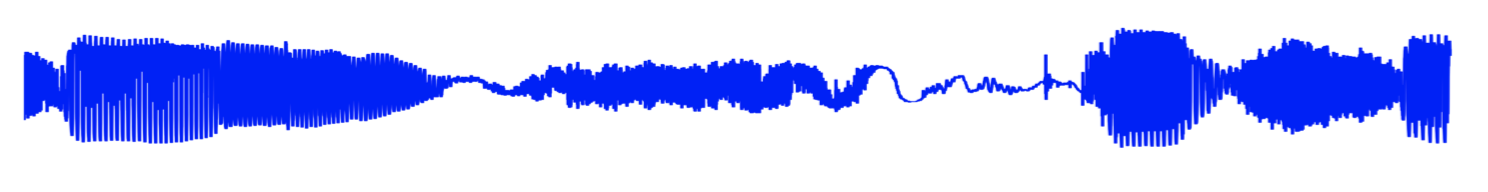
\includegraphics[width=0.9\linewidth]{figs/wavenet_ex.png}
	\end{figure}
	\begin{block}{Solution}
		Autoregressive model
		\vspace{-0.3cm}
		\[
		    p(\bx| \btheta) = \prod_{t=1}^T p(x_t|\bx_{1:t-1}, \btheta).
		\]
		\vspace{-0.3cm}
	\end{block}
	\begin{itemize}
		\item Each conditional $p(x_t|\bx_{1:t-1}, \btheta)$ models the distribution for the timestamp $t$.
		\item The model uses \textbf{causal} dilated convolutions.
	\end{itemize}
	\myfootnotewithlink{https://arxiv.org/abs/1609.03499}{Oord A. et al. Wavenet: A generative model for raw audio, 2016}
\end{frame}
%=======
\begin{frame}{WaveNet}
	\begin{figure}
	    \centering
	    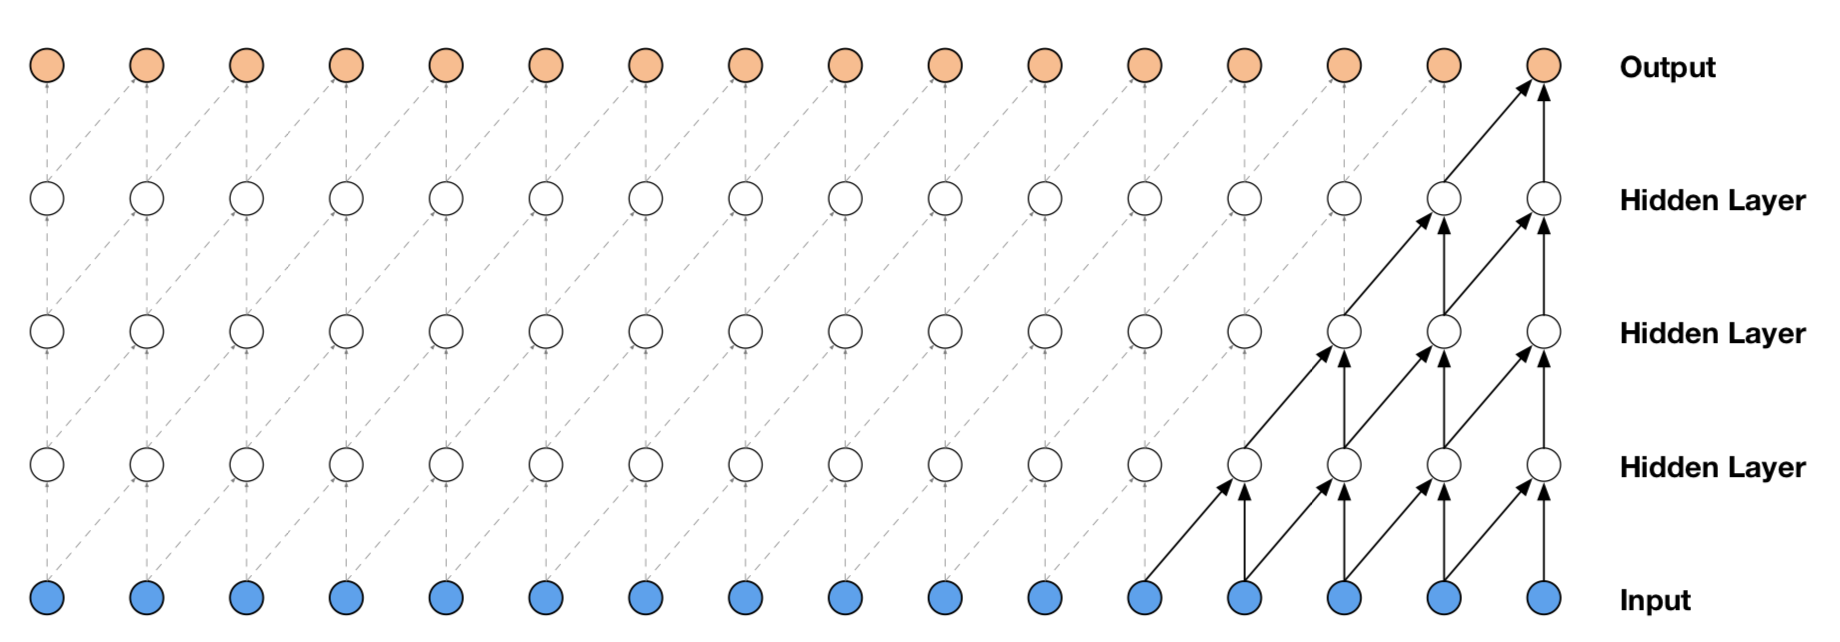
\includegraphics[width=0.9\linewidth]{figs/wavenet1.png}
	\end{figure}
	
	\begin{figure}
	    \centering
	    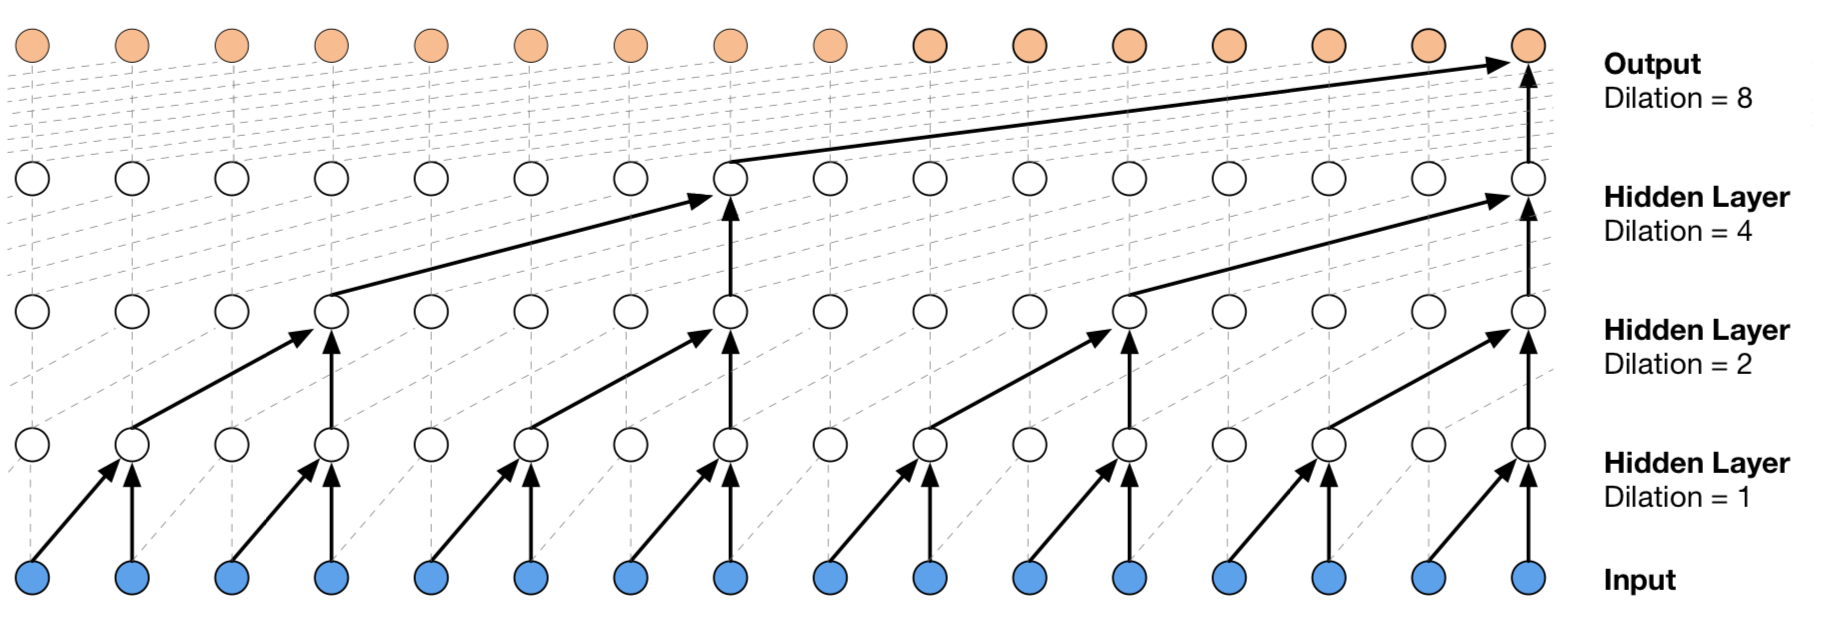
\includegraphics[width=0.9\linewidth]{figs/wavenet2.png}
	\end{figure}
	\myfootnotewithlink{https://arxiv.org/abs/1609.03499}{Oord A. et al. Wavenet: A generative model for raw audio, 2016}
\end{frame}
%=======
\begin{frame}{PixelCNN}
	\begin{block}{Goal}
		Model a distribution $\pi(\bx)$ of natural images.
	\end{block}
	\begin{block}{Solution}
		Autoregressive model on 2D pixels
		\[
		    p(\bx | \btheta) = \prod_{j=1}^{\text{width} \times \text{height}} p(x_j|\bx_{1:j-1}, \btheta).
		\]
		\begin{itemize}
			\item We need to introduce the ordering of image pixels.
		    \item The convolution should be \textbf{masked} to make them causal.
		    \item The image has RGB channels, these dependencies could be addressed.
		\end{itemize}
	\end{block}
	\myfootnotewithlink{https://arxiv.org/abs/1601.06759}{Oord A., Kalchbrenner N., Kavukcuoglu K. Pixel recurrent neural networks, 2016}
\end{frame}
%=======
\begin{frame}{PixelCNN}
	\begin{minipage}[t]{0.5\columnwidth}
		\begin{block}{Raster ordering}
			\begin{figure}
				\centering
		        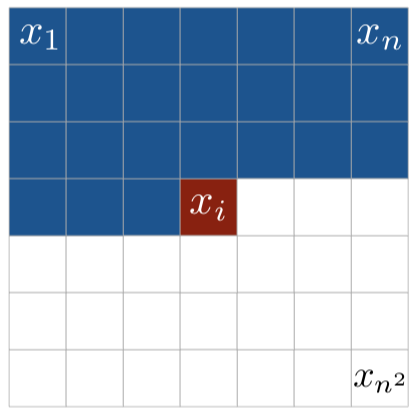
\includegraphics[width=0.7\linewidth]{figs/pixelcnn1.png}
			\end{figure}
		\end{block}
		\vspace{-0.5cm}
		\begin{block}{Masked convolution kernel}
			\begin{figure}
				\centering
		        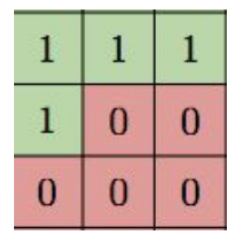
\includegraphics[width=0.35\linewidth]{figs/pixelcnn_0_1.png}
			\end{figure}
		\end{block}
	\end{minipage}%
	\begin{minipage}[t]{0.5\columnwidth}
		\begin{block}{Dependencies between pixels}
			\begin{figure}
				\centering
		        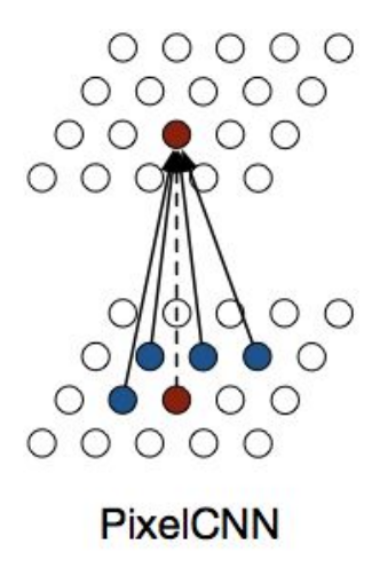
\includegraphics[width=0.5\linewidth]{figs/pixelcnn_0_2.png}
			\end{figure}
			\vspace{-0.3cm}
			\begin{figure}
				\centering
		        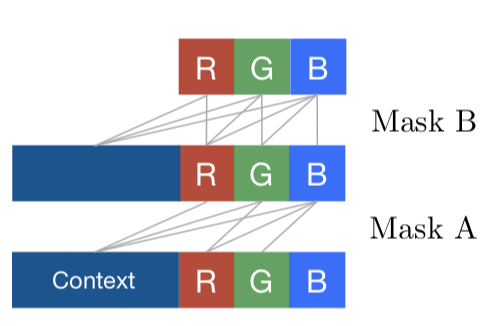
\includegraphics[width=0.65\linewidth]{figs/pixelcnn2.png}
			\end{figure}
		\end{block}
	\end{minipage}
	\myfootnotewithlink{https://arxiv.org/abs/1601.06759}{Oord A., Kalchbrenner N., Kavukcuoglu K. Pixel recurrent neural networks, 2016}
\end{frame}
%=======
\begin{frame}{PixelCNN}
	\begin{block}{CIFAR-10 generated samples}
		\vspace{-0.2cm}
		\begin{figure}
			\centering
	  		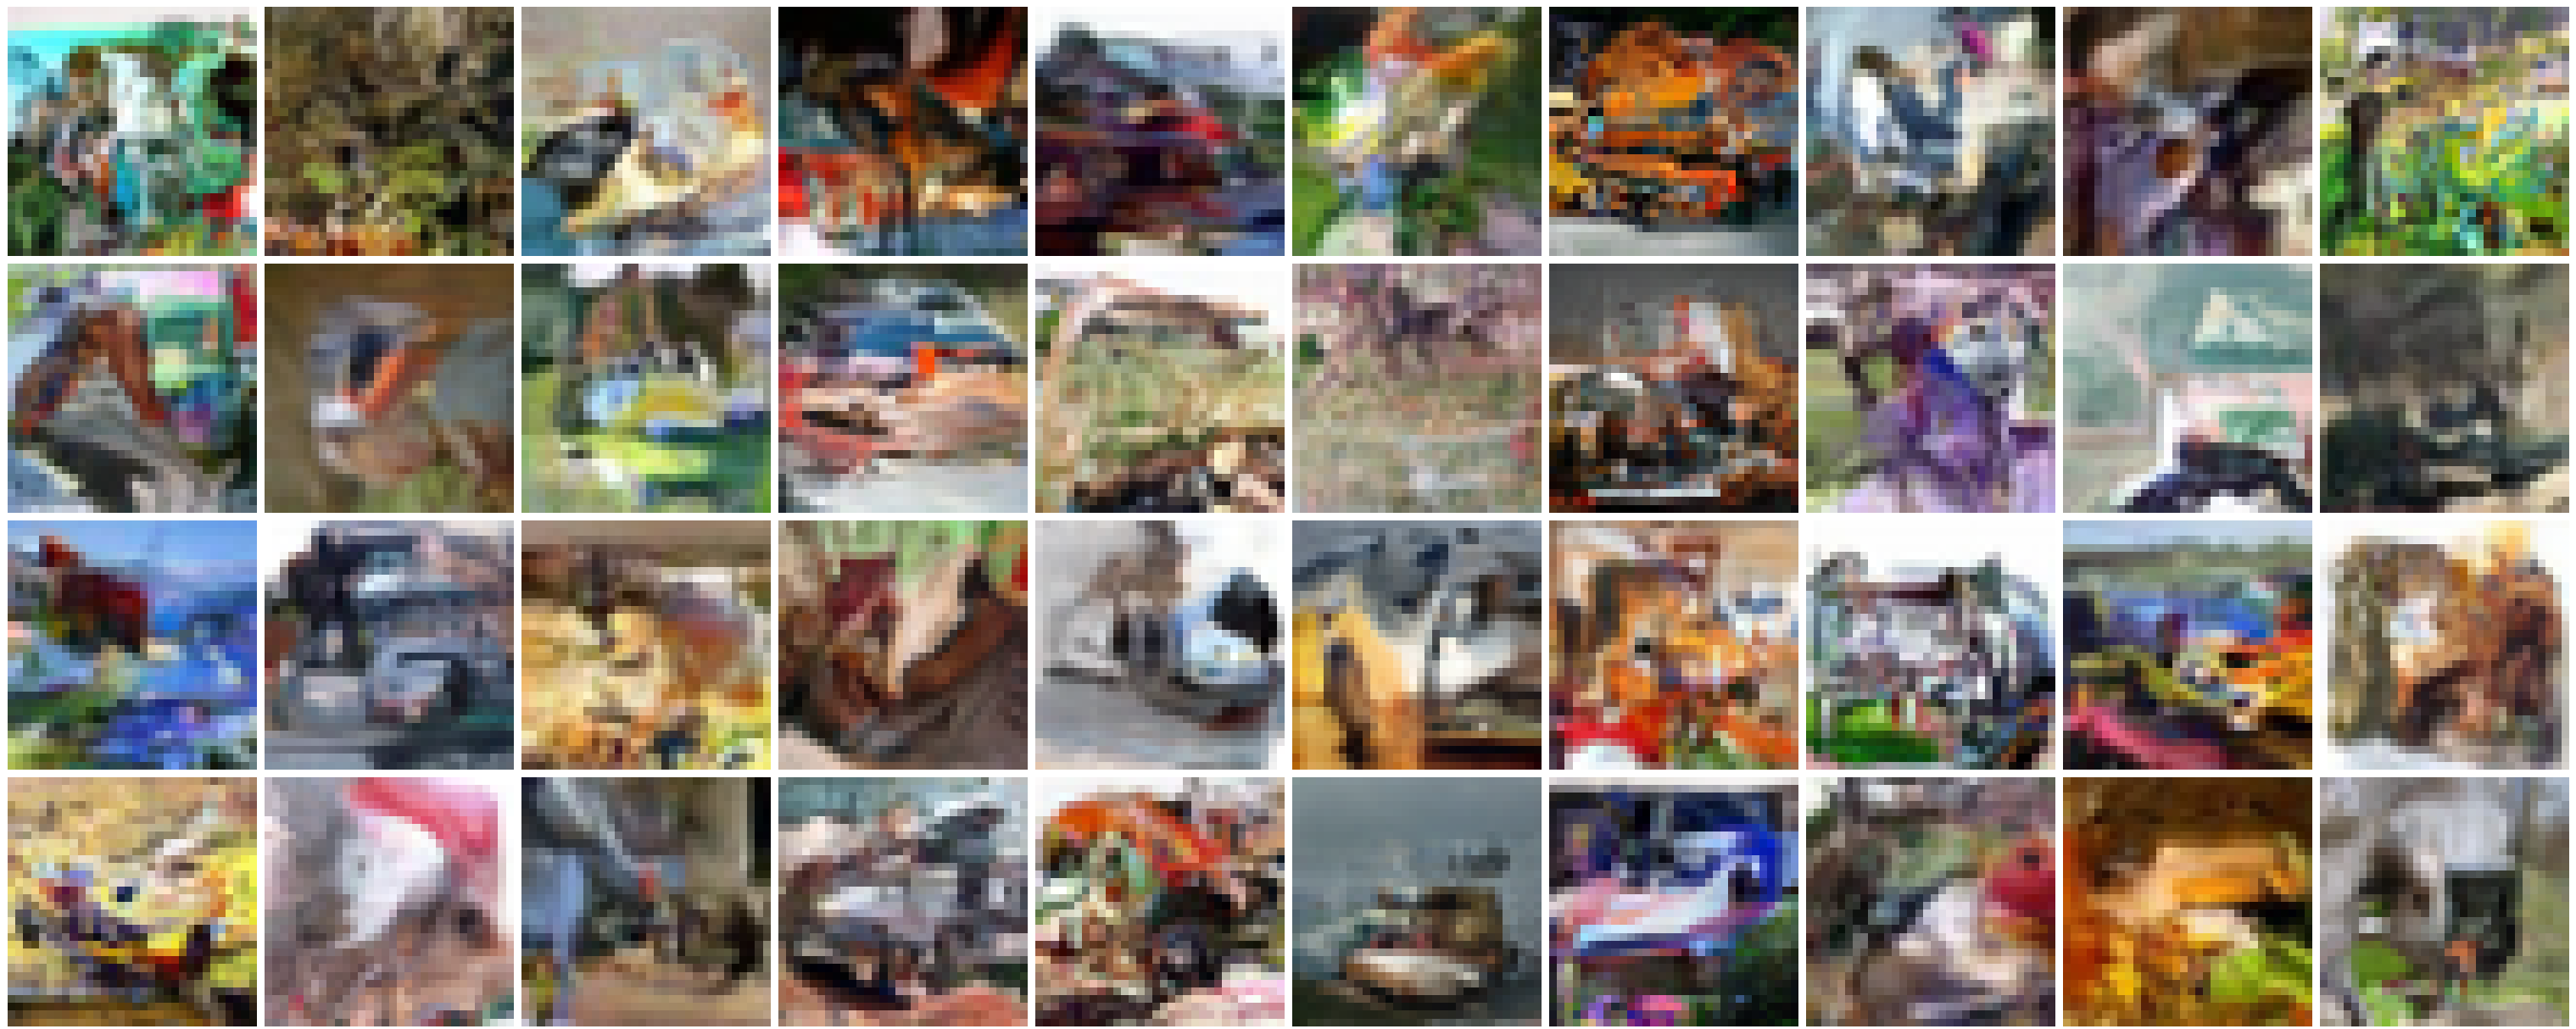
\includegraphics[width=0.7\linewidth]{figs/pixelcnn_results}
		\end{figure}
	\end{block}
	\vspace{-0.2cm}
	\begin{block}{CIFAR-10 perfomance}
		\begin{figure}
			\centering
	  		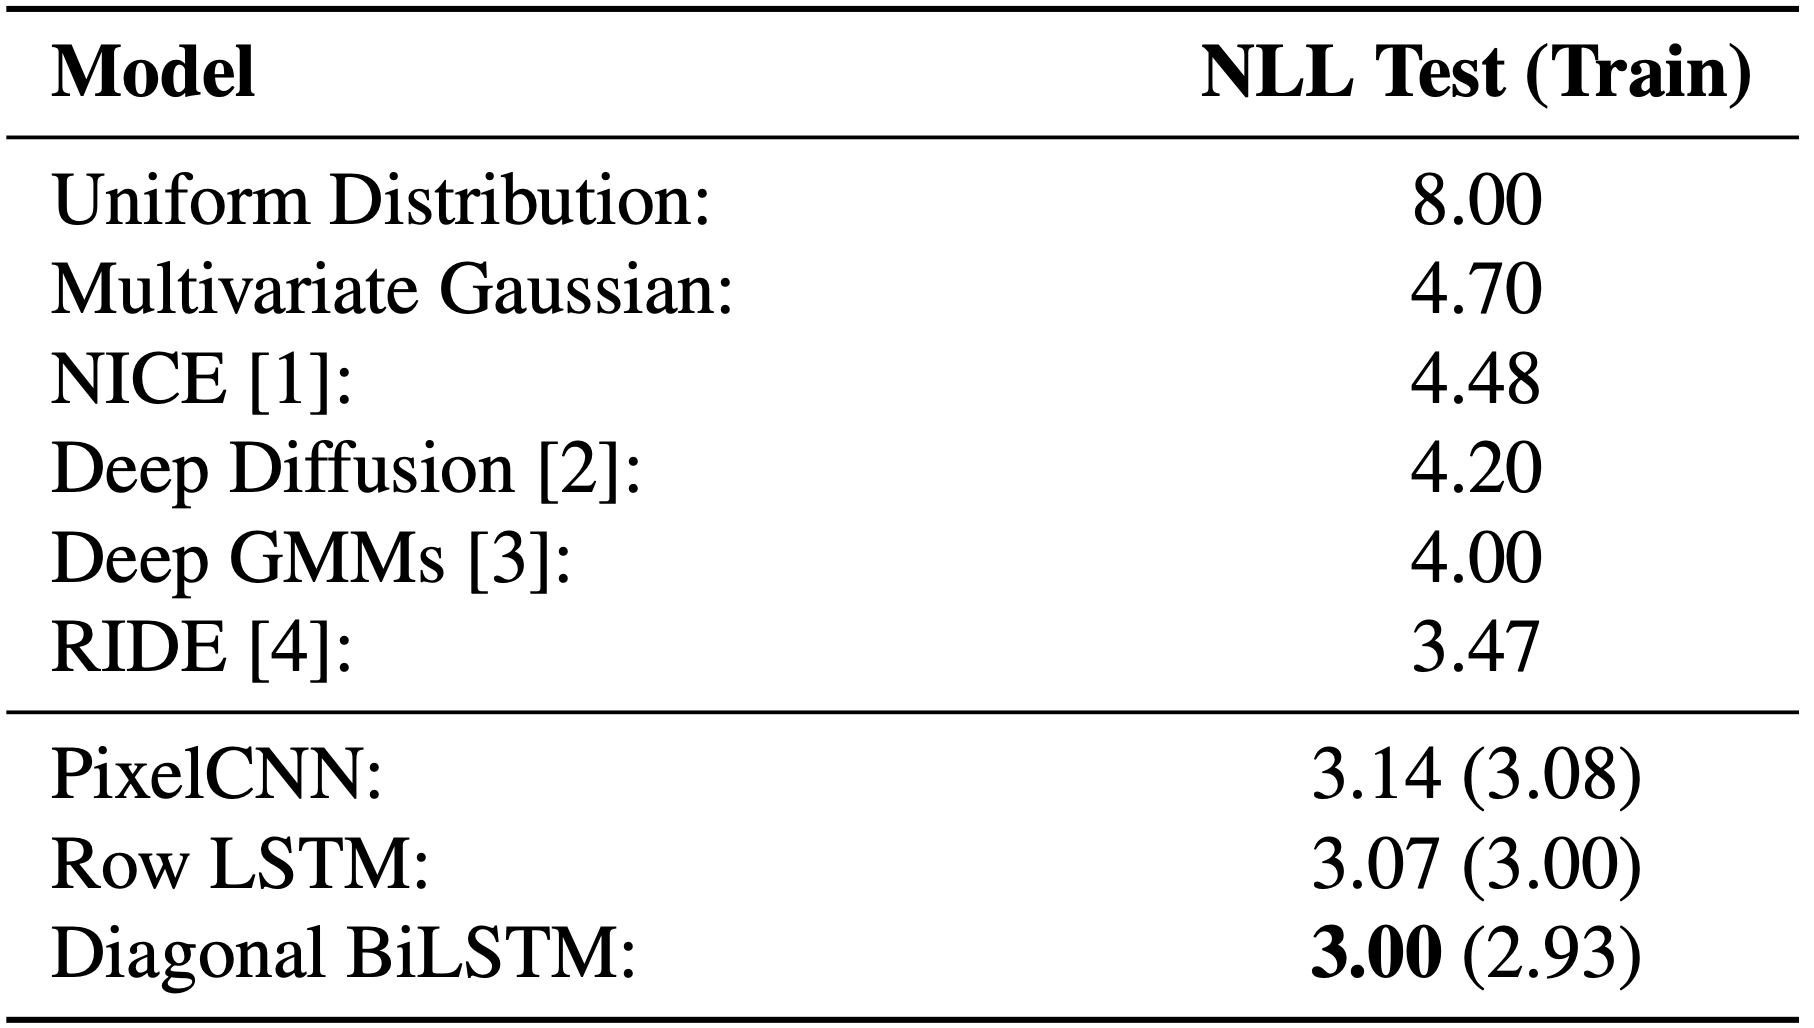
\includegraphics[width=0.45\linewidth]{figs/pixelcnn_results2}
		\end{figure}
	\end{block}
	\myfootnotewithlink{https://arxiv.org/abs/1601.06759}{Oord A., Kalchbrenner N., Kavukcuoglu K. Pixel recurrent neural networks, 2016}
\end{frame}
%=======
\begin{frame}{PixelCNN++}
	\begin{block}{CIFAR-10 pixel values distribution}
		\begin{figure}
			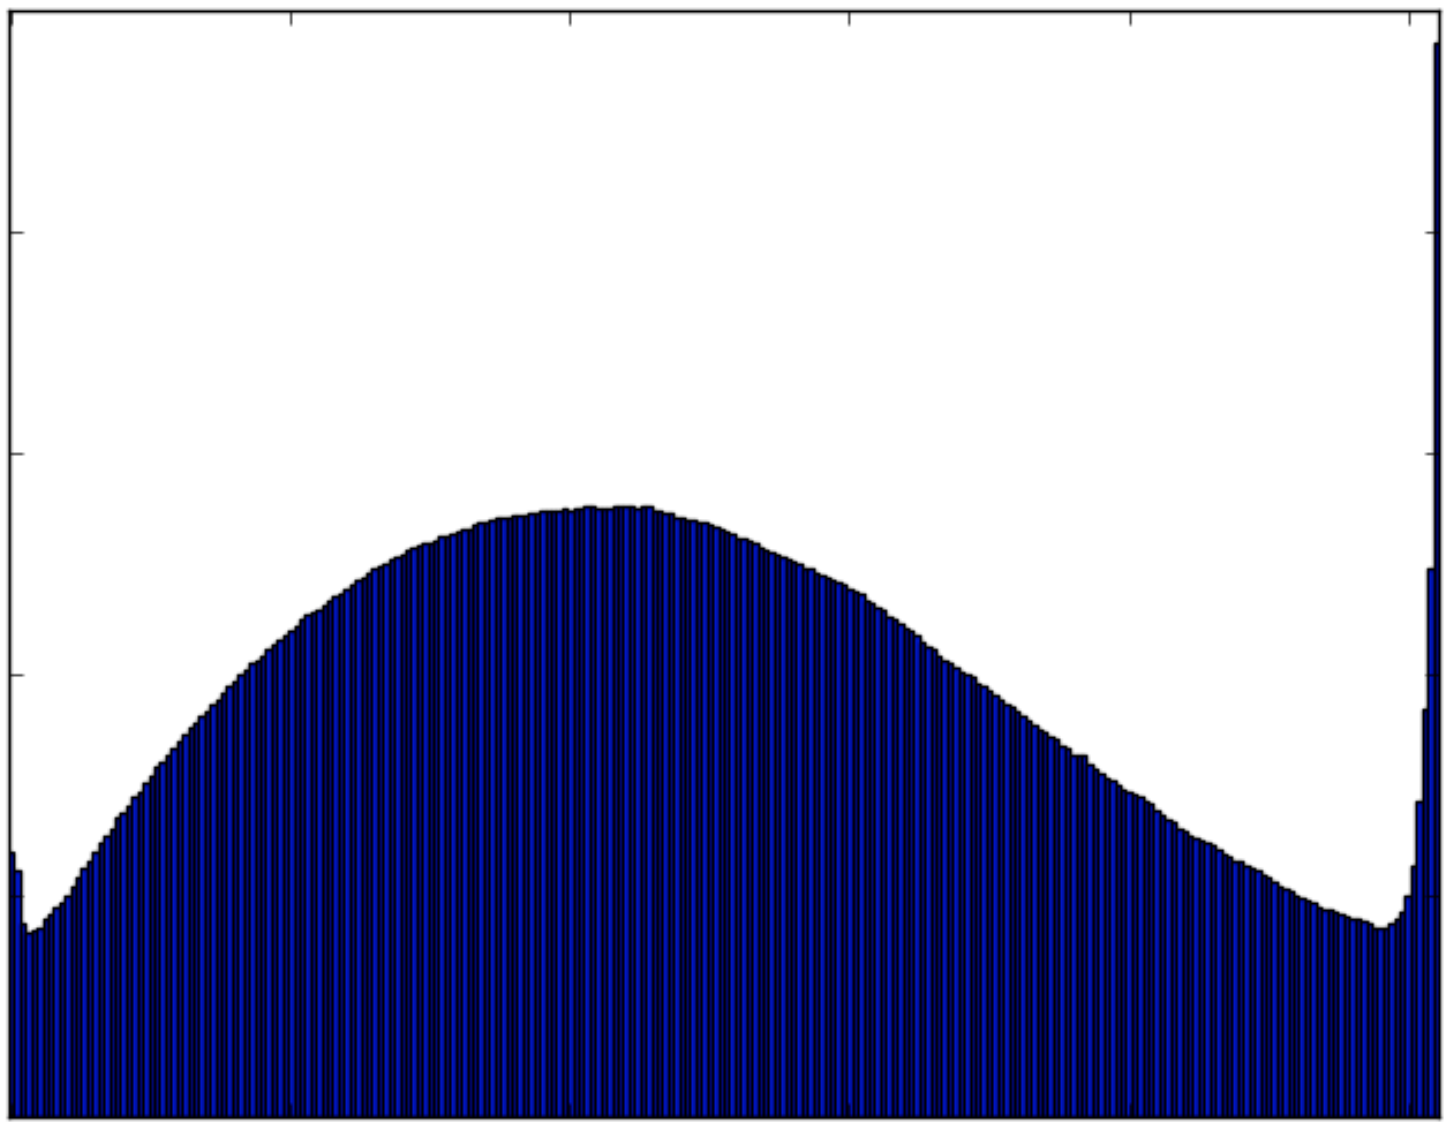
\includegraphics[width=0.3\linewidth]{figs/pixelcnn++_pixels_distr}
		\end{figure}
	\end{block}
	\vspace{-0.5cm}
	\begin{itemize}
		\item Standard PixelCNN outputs softmax probabilities for values $\{0, 255\}$ (256 outputs feature maps). 
		\item Categorical distribution do not know anything about numerical relationships (220 is close to 221 and far from 15).
		\item If pixel value is not presented in the training dataset, it won't be predicted.
		\item (Look at the edges of the distributions: they have higher probability mass).
	\end{itemize}
	\myfootnotewithlink{https://arxiv.org/abs/1701.05517}{Salimans T. et al. PixelCNN++: Improving the PixelCNN with Discretized Logistic Mixture Likelihood and Other Modifications, 2017}
\end{frame}
%=======
\begin{frame}{PixelCNN++}
		\begin{minipage}[t]{0.55\columnwidth}
		\begin{block}{Mixture of logistic distributions}
			\begin{align*}
				p(x | \mu, s) &= \frac{\exp^{-(x - \mu) / s}}{s (1 + \exp^{-(x - \mu) / s})^2}; \\
				p(x | \bmu, \bs, \bpi) &= \sum_{k=1}^K \pi_k p(x | \mu_k, s_k);
			\end{align*}
		\end{block}
		\end{minipage}%
		\begin{minipage}[t]{0.45\columnwidth}
				\begin{figure}
					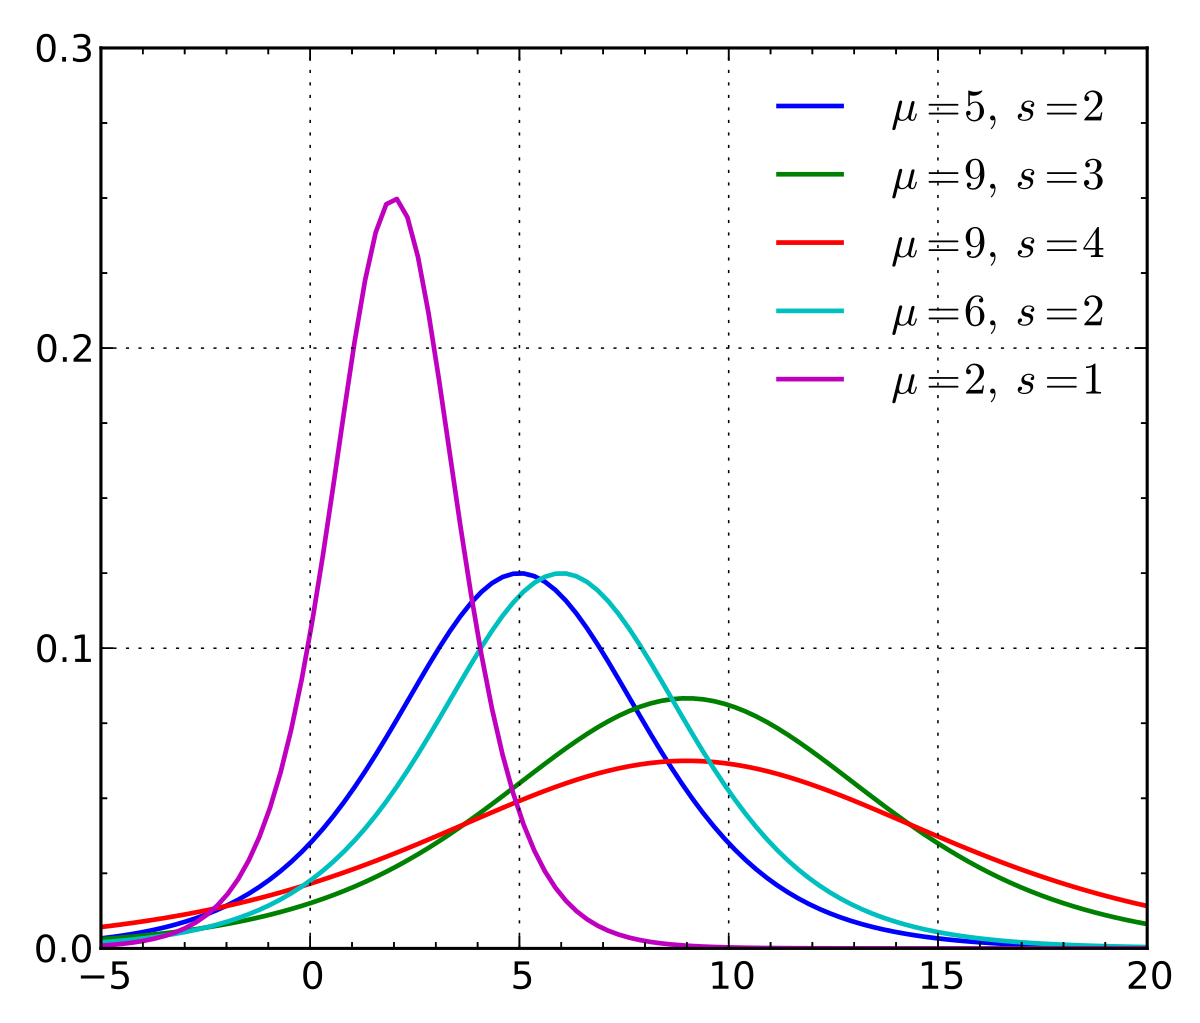
\includegraphics[width=\linewidth]{figs/picelcnn++logistic}
				\end{figure}
		\end{minipage}
	To adopt probability calculation to discrete values:
	\[
		P_d(x | \bmu, \bs, \bpi) = P(x + 0.5 | \bmu, \bs, \bpi) - P(x - 0.5 | \bmu, \bs, \bpi)
	\]
	For the edge case of 0, replace $x - 0.5$ by $-\infty$, and for 255 replace $x + 0.5$ by $+\infty$.
	\myfootnotewithlink{https://arxiv.org/abs/1701.05517}{Salimans T. et al. PixelCNN++: Improving the PixelCNN with Discretized Logistic Mixture Likelihood and Other Modifications, 2017}
\end{frame}
%=======
\begin{frame}{PixelCNN++}
	\begin{block}{CIFAR-10 generated samples}
		\begin{figure}
			\centering
	  		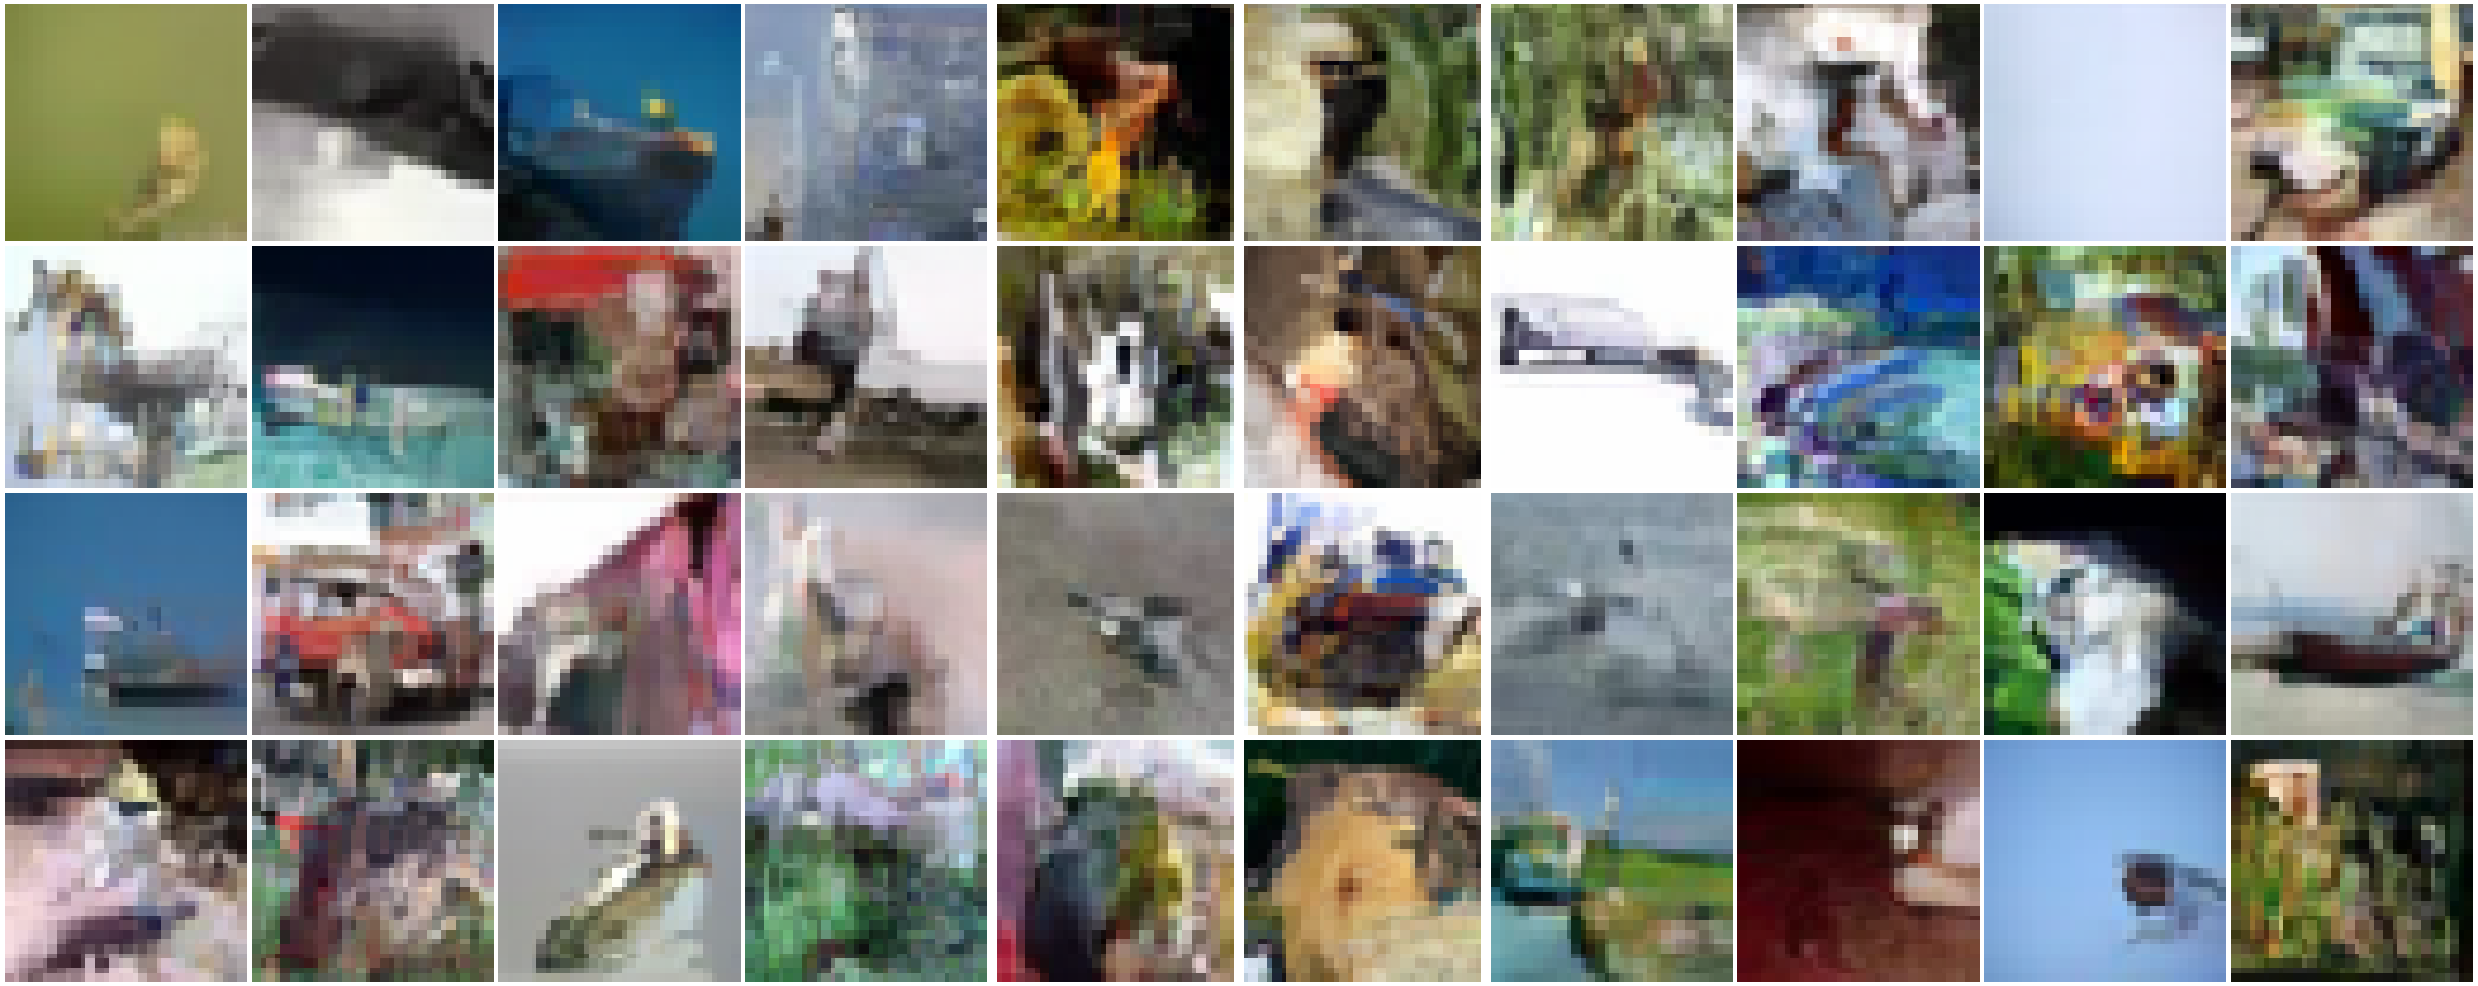
\includegraphics[width=0.7\linewidth]{figs/pixelcnn++samples}
		\end{figure}
	\end{block}
	\vspace{-0.2cm}
	\begin{block}{CIFAR-10 perfomance}
		\vspace{-0.3cm}
		\begin{figure}
			\centering
	  		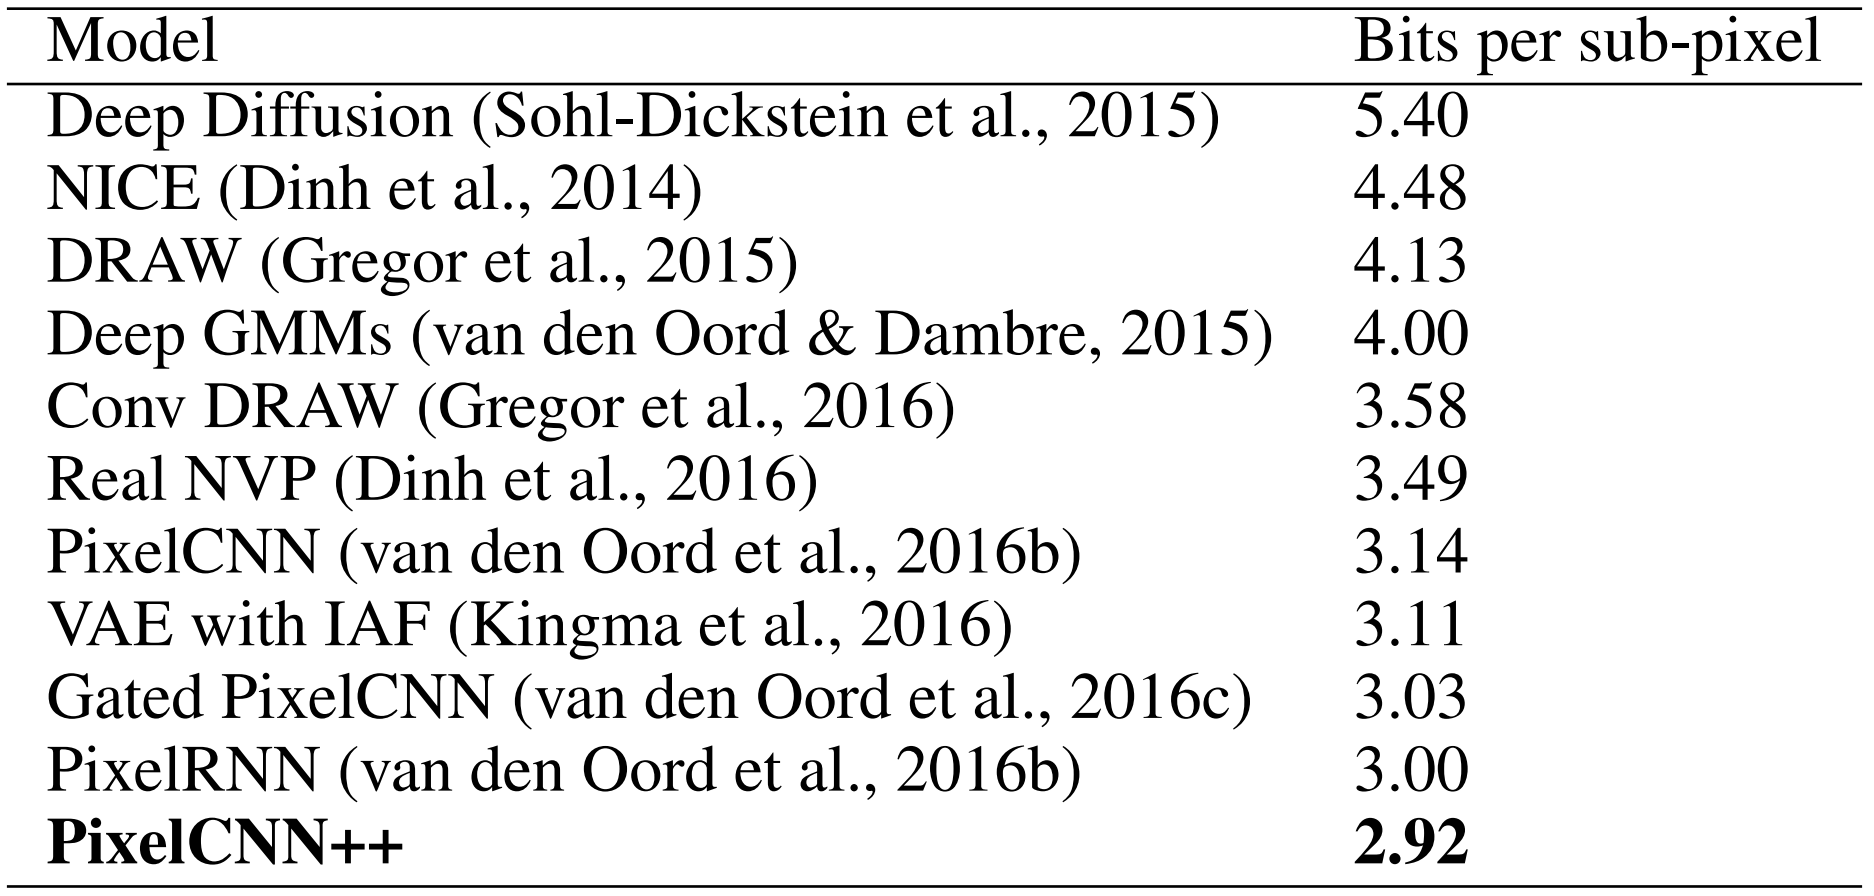
\includegraphics[width=0.5\linewidth]{figs/pixelcnn++results}
		\end{figure}
	\end{block}
	\myfootnotewithlink{https://arxiv.org/abs/1701.05517}{Salimans T. et al. PixelCNN++: Improving the PixelCNN with Discretized Logistic Mixture Likelihood and Other Modifications, 2017}
\end{frame}
%=======
\begin{frame}{Generative models zoo}
	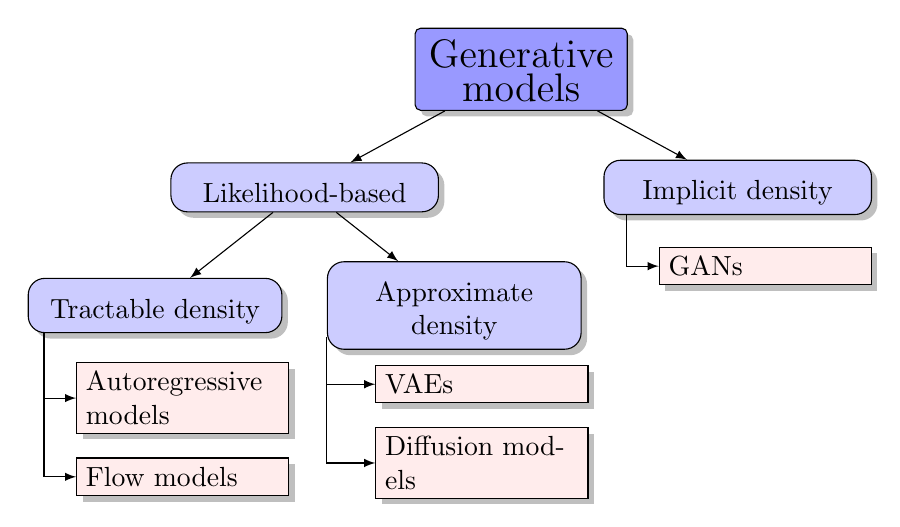
\begin{tikzpicture}[
	 	basic/.style  = {draw, text width=2cm, drop shadow, rectangle},
	 	root/.style   = {basic, rounded corners=2pt, thin, text height=1.1em, text width=7em, align=center, fill=blue!40},
	 	level 1/.style={sibling distance=55mm},
	 	level 2/.style = {basic, rounded corners=6pt, thin, align=center, fill=blue!20, text height=1.1em, text width=9em, sibling distance=38mm},
	 	level 3/.style = {basic, rounded corners=6pt, thin,align=center, fill=blue!20, text width=8.5em},
	 	level 4/.style = {basic, thin, align=left, fill=pink!30, text width=7em},
		edge from parent/.style={->,draw},
		>=latex]
		
		% root of the the initial tree, level 1
		\node[root] {\Large Generative models}
		% The first level, as children of the initial tree
		child {node[level 2] (c1) {Likelihood-based}
			child {node[level 3] (c11) {Tractable density}}
			child {node[level 3] (c12) {Approximate density}}
		}
		child {node[level 2] (c2) {Implicit density}};
		
		% The second level, relatively positioned nodes
		\begin{scope}[every node/.style={level 4}]
		\node [below of = c11, yshift=-5pt, xshift=10pt] (c111) {Autoregressive models};
		\node [below of = c111] (c112) {Flow models};
		
		\node [below of = c12, xshift=10pt] (c121) {VAEs};
		\node [below of = c121] (c122) {Diffusion models};
		
		\node [below of = c2, xshift=10pt] (c21) {GANs};
		\end{scope}
		
		% lines from each level 1 node to every one of its "children"
		\foreach \value in {1,2}
		\draw[->] (c11.194) |- (c11\value.west);
		
		\foreach \value in {1,2}
		\draw[->] (c12.194) |- (c12\value.west);
		
		\draw[->] (c2.194) |- (c21.west);
		
	\end{tikzpicture}
\end{frame}
%=======
\begin{frame}{Bayesian framework}
	\begin{block}{Bayes theorem}
		\[
			p(\bt | \bx) = \frac{p(\bx | \bt) p(\bt)}{p(\bx)} = \frac{p(\bx | \bt) p(\bt)}{\int p(\bx | \bt) p(\bt) d \bt} 
		\]
		\begin{itemize}
			\item $\bx$ -- observed variables, $\bt$ -- unobserved variables (latent variables/parameters);
			\item $p(\bx | \bt)$ -- likelihood;
			\item $p(\bx) = \int p(\bx | \bt) p(\bt) d \bt$ -- evidence;
			\item $p(\bt)$ -- prior distribution, $p(\bt | \bx)$ -- posterior distribution.
		\end{itemize}
	\end{block}
	\begin{block}{Meaning}
		We have unobserved variables $\bt$ and some prior knowledge about them $p(\bt)$. Then, the data $\bx$ has been observed. 
		Posterior distribution $p(\bt | \bx)$ summarizes the knowledge after the observations.
	\end{block}
\end{frame}
%=======
\begin{frame}{Bayesian framework}
	Let consider the case, where the unobserved variables $\bt$ is our model parameters $\btheta$.
	\begin{itemize}
		\item $\bX = \{\bx_i\}_{i=1}^n$ -- observed samples;
		\item $p(\btheta)$ -- prior parameters distribution (we treat model parameters $\btheta$ as random variables).
	\end{itemize}
	\begin{block}{Posterior distribution}
		\[
			p(\btheta | \bX) = \frac{p(\bX | \btheta) p(\btheta)}{p(\bX)} = \frac{p(\bX | \btheta) p(\btheta)}{\int p(\bX | \btheta) p(\btheta) d \btheta} 
		\]
		\vspace{-0.2cm}
	\end{block}
	\begin{block}{Bayesian inference}
		\vspace{-0.2cm}
		\[
			p(\bx | \bX) = \int p(\bx | \btheta) p(\btheta | \bX) d \btheta
		\]
	\end{block}
 	Note the difference from
	 	\[
	 		p(\bx) = \int p(\bx | \btheta) p(\btheta) d \btheta.
	 	\]
\end{frame}
%=======
\begin{frame}{Bayesian framework}
	\begin{block}{Posterior distribution}
		\[
		p(\btheta | \bX) = \frac{p(\bX | \btheta) p(\btheta)}{p(\bX)} = \frac{p(\bX | \btheta) p(\btheta)}{\int p(\bX | \btheta) p(\btheta) d \btheta} 
		\]
		\vspace{-0.2cm}
	\end{block}
	\begin{block}{Bayesian inference}
		\vspace{-0.2cm}
		\[
		p(\bx | \bX) = \int p(\bx | \btheta) p(\btheta | \bX) d \btheta
		\]
	\end{block}
	If evidence $p(\bX)$ is intractable (due to multidimensional integration), we can't get posterior distribution and perform the precise inference.
    \begin{block}{Maximum a posteriori (MAP) estimation}
    \vspace{-0.2cm}
    \[
        \btheta^* = \argmax_{\btheta} p(\btheta | \bX) = \argmax_{\btheta} \bigl(\log p(\bX | \btheta) + \log p(\btheta) \bigr)
    \]
    \end{block}
\end{frame}
%=======
\begin{frame}{Bayesian framework}
	\begin{block}{MAP estimation}
		\vspace{-0.2cm}
		\[
		\btheta^* = \argmax_{\btheta} p(\btheta | \bX) = \argmax_{\btheta} \bigl(\log p(\bX | \btheta) + \log p(\btheta) \bigr)
		\]
	\end{block}
	Estimated $\btheta^*$ is a deterministic variable, but we could treat it as a random variable with density $p(\btheta | \bX) = \delta(\btheta - \btheta^*)$.
	\begin{block}{Dirac delta function}
		\[
			\delta(x) = 
			\begin{cases}
				+\infty, \quad x = 0; \\
				0, \quad x \neq 0;
			\end{cases} \, 
			\int \delta(x) dx = 1; \,\, 
			\int f(x) \delta (x - y) dx = f(y).
		\]
	\end{block}
	\begin{block}{MAP inference}
		\[
			p(\bx | \bX) = \int p(\bx| \btheta) p(\btheta | \bX ) d \btheta \approx p(\bx | \btheta^*).
		\]
	\end{block}
\end{frame}
%=======
\begin{frame}{Summary}
	\begin{itemize}
		\item MADE model is an autoregressive autoencoder with masked dense layers.
		\vfill
		\item WaveNet and PixelCNN models use masked causal convolutions (1D or 2D) to get autoregressize model.
		\vfill
		\item PixelCNN++ proposes to use discretized mixture of logistics for output distribution.
		\vfill
		\item Bayesian inference is a generalization of most common machine learning tasks. It allows to construct MLE, MAP and bayesian inference, to compare models complexity and many-many more cool stuff.
	\end{itemize}
\end{frame}
\end{document} 